%%
%% Copyright 2007, 2008, 2009 Elsevier Ltd
%%
%% This file is part of the 'Elsarticle Bundle'.
%% ---------------------------------------------
%%
%% It may be distributed under the conditions of the LaTeX Project Public
%% License, either version 1.2 of this license or (at your option) any
%% later version.  The latest version of this license is in
%%    http://www.latex-project.org/lppl.txt
%% and version 1.2 or later is part of all distributions of LaTeX
%% version 1999/12/01 or later.
%%
%% The list of all files belonging to the 'Elsarticle Bundle' is
%% given in the file `manifest.txt'.
%%
\documentclass[5p,,preprint,12pt,twocolumn]{elsarticle}
\makeatletter\if@twocolumn\PassOptionsToPackage{switch}{lineno}\else\fi\makeatother


\usepackage{tabulary,xcolor}
\usepackage{amsfonts,amsmath,amssymb}
\usepackage[T1]{fontenc}
\makeatletter
\let\save@ps@pprintTitle\ps@pprintTitle
\def\ps@pprintTitle{\save@ps@pprintTitle\gdef\@oddfoot{\footnotesize\itshape \null\hfill\today}}
\def\hlinewd#1{%
  \noalign{\ifnum0=`}\fi\hrule \@height #1%
  \futurelet\reserved@a\@xhline}
\def\tbltoprule{\hlinewd{.8pt}\\[-12pt]}
\def\tblbottomrule{\noalign{\vspace*{6pt}}\hline\noalign{\vspace*{2pt}}}
\def\tblmidrule{\noalign{\vspace*{6pt}}\hline\noalign{\vspace*{2pt}}}
\AtBeginDocument{\ifNAT@numbers \biboptions{sort&compress}\fi}
\makeatother

  


\usepackage{ifluatex}
\ifluatex
\usepackage{fontspec}
\defaultfontfeatures{Ligatures=TeX}
\usepackage[]{unicode-math}
\unimathsetup{math-style=TeX}
\else 
\usepackage[utf8]{inputenc}
\fi 
\ifluatex\else\usepackage{stmaryrd}\fi

  
%%%%%%%%%%%%%%%%%%%%%%%%%%%%%%%%%%%%%%%%%%%%%%%%%%%%%%%%%%%%%%%%%%%%%%%%%%
% Following additional macros are required to function some 
% functions which are not available in the class used.
%%%%%%%%%%%%%%%%%%%%%%%%%%%%%%%%%%%%%%%%%%%%%%%%%%%%%%%%%%%%%%%%%%%%%%%%%%
\usepackage{url,multirow,morefloats,floatflt,cancel,tfrupee}
\makeatletter


\AtBeginDocument{\@ifpackageloaded{textcomp}{}{\usepackage{textcomp}}}
\makeatother
\usepackage{colortbl}
\usepackage{xcolor}
\usepackage{pifont}
\usepackage[nointegrals]{wasysym}
\urlstyle{rm}
\makeatletter

%%%For Table column width calculation.
\def\mcWidth#1{\csname TY@F#1\endcsname+\tabcolsep}

%%Hacking center and right align for table
\def\cAlignHack{\rightskip\@flushglue\leftskip\@flushglue\parindent\z@\parfillskip\z@skip}
\def\rAlignHack{\rightskip\z@skip\leftskip\@flushglue \parindent\z@\parfillskip\z@skip}

%Etal definition in references
\@ifundefined{etal}{\def\etal{\textit{et~al}}}{}


%\if@twocolumn\usepackage{dblfloatfix}\fi
\usepackage{ifxetex}
\ifxetex\else\if@twocolumn\@ifpackageloaded{stfloats}{}{\usepackage{dblfloatfix}}\fi\fi

\AtBeginDocument{
\expandafter\ifx\csname eqalign\endcsname\relax
\def\eqalign#1{\null\vcenter{\def\\{\cr}\openup\jot\m@th
  \ialign{\strut$\displaystyle{##}$\hfil&$\displaystyle{{}##}$\hfil
      \crcr#1\crcr}}\,}
\fi
}

%For fixing hardfail when unicode letters appear inside table with endfloat
\AtBeginDocument{%
  \@ifpackageloaded{endfloat}%
   {\renewcommand\efloat@iwrite[1]{\immediate\expandafter\protected@write\csname efloat@post#1\endcsname{}}}{\newif\ifefloat@tables}%
}%

\def\BreakURLText#1{\@tfor\brk@tempa:=#1\do{\brk@tempa\hskip0pt}}
\let\lt=<
\let\gt=>
\def\processVert{\ifmmode|\else\textbar\fi}
\let\processvert\processVert

\@ifundefined{subparagraph}{
\def\subparagraph{\@startsection{paragraph}{5}{2\parindent}{0ex plus 0.1ex minus 0.1ex}%
{0ex}{\normalfont\small\itshape}}%
}{}

% These are now gobbled, so won't appear in the PDF.
\newcommand\role[1]{\unskip}
\newcommand\aucollab[1]{\unskip}
  
\@ifundefined{tsGraphicsScaleX}{\gdef\tsGraphicsScaleX{1}}{}
\@ifundefined{tsGraphicsScaleY}{\gdef\tsGraphicsScaleY{.9}}{}
% To automatically resize figures to fit inside the text area
\def\checkGraphicsWidth{\ifdim\Gin@nat@width>\linewidth
	\tsGraphicsScaleX\linewidth\else\Gin@nat@width\fi}

\def\checkGraphicsHeight{\ifdim\Gin@nat@height>.9\textheight
	\tsGraphicsScaleY\textheight\else\Gin@nat@height\fi}

\def\fixFloatSize#1{}%\@ifundefined{processdelayedfloats}{\setbox0=\hbox{\includegraphics{#1}}\ifnum\wd0<\columnwidth\relax\renewenvironment{figure*}{\begin{figure}}{\end{figure}}\fi}{}}
\let\ts@includegraphics\includegraphics

\def\inlinegraphic[#1]#2{{\edef\@tempa{#1}\edef\baseline@shift{\ifx\@tempa\@empty0\else#1\fi}\edef\tempZ{\the\numexpr(\numexpr(\baseline@shift*\f@size/100))}\protect\raisebox{\tempZ pt}{\ts@includegraphics{#2}}}}

%\renewcommand{\includegraphics}[1]{\ts@includegraphics[width=\checkGraphicsWidth]{#1}}
\AtBeginDocument{\def\includegraphics{\@ifnextchar[{\ts@includegraphics}{\ts@includegraphics[width=\checkGraphicsWidth,height=\checkGraphicsHeight,keepaspectratio]}}}

\DeclareMathAlphabet{\mathpzc}{OT1}{pzc}{m}{it}

\def\URL#1#2{\@ifundefined{href}{#2}{\href{#1}{#2}}}

%%For url break
\def\UrlOrds{\do\*\do\-\do\~\do\'\do\"\do\-}%
\g@addto@macro{\UrlBreaks}{\UrlOrds}



\edef\fntEncoding{\f@encoding}
\def\EUoneEnc{EU1}
\makeatother
\def\floatpagefraction{0.8} 
\def\dblfloatpagefraction{0.8}
\def\style#1#2{#2}
\def\xxxguillemotleft{\fontencoding{T1}\selectfont\guillemotleft}
\def\xxxguillemotright{\fontencoding{T1}\selectfont\guillemotright}

\newif\ifmultipleabstract\multipleabstractfalse%
\newenvironment{typesetAbstractGroup}{}{}%

%%%%%%%%%%%%%%%%%%%%%%%%%%%%%%%%%%%%%%%%%%%%%%%%%%%%%%%%%%%%%%%%%%%%%%%%%%
\emergencystretch 20pt \tolerance = 1500 \def\floatpagefraction{0.8}




%%%%%%%%%%%%%%%%%%%%%%%%%%%%%%%%%%%%%%%%%%
% Feature enabled:
%toc: yes
%bookmark: yes
%pagenum: yes
%text-layout: twocolumn
%endfloat: placeins
%%%%%%%%%%%%%%%%%%%%%%%%%%%%%%%%%%%%%%%%%%
\makeatletter
\@ifpackageloaded{hyperref}{\def\alreadybookmark{}}{\usepackage[hidelinks]{hyperref}}
\@ifpackageloaded{bookmark}{}{\usepackage{bookmark}}
\makeatother
\ifdefined\alreadybookmark\def\pdfbookmark[#1]#2#3{}\fi
\makeatletter
\def\ps@pprintTitle{\save@ps@pprintTitle\gdef\@oddfoot{\footnotesize\hspace*{.5\textwidth}\thepage\itshape \null\hfill\today}}
\makeatother
          \makeatletter\@ifundefined{tableofcontents}{\usepackage{typeset-custom-toc}}{}\makeatother
\usepackage[section]{placeins}

\usepackage{etoolbox}

\usepackage{longtable}

\usepackage{float}

\makeatletter
\AtBeginDocument{\@ifpackageloaded{rotating}{\PassOptionsToPackage{figuresright}{rotating}}{\usepackage[figuresright]{rotating}}\setlength{\rotFPtop}{0pt plus 1fil}\setlength{\rotFPbot}{0pt plus 1fil}}
\makeatother

\makeatletter
 \AtBeginDocument{%
  \@ifpackagewith{endfloat}{figuresonly}
  {\DeclareDelayedFloatFlavor{sidewaysfigure}{figure}}%true
  {\@ifpackagewith{endfloat}{tablesonly}{\DeclareDelayedFloatFlavor{sidewaystable}{table}\DeclareDelayedFloatFlavor{longtable}{table}\DeclareDelayedFloatFlavor{landscape}{table}}%true
  {\@ifpackageloaded{endfloat}{\DeclareDelayedFloatFlavor{sidewaysfigure}{figure}\DeclareDelayedFloatFlavor{sidewaystable}{table}\DeclareDelayedFloatFlavor{longtable}{table}\DeclareDelayedFloatFlavor{landscape}{table}}{}}%false
  }%false
  }
\makeatother

\usepackage{pdflscape}

\begin{document}
\pdfbookmark[title]{Polymers for Near-field Electrospinning with Spatial Control}{title}


\begin{frontmatter}
	
\title{Polymers for Near-field Electrospinning with Spatial Control
}
    
\author[]{Antonio Osamu Katagiri Tanaka}
\ead{oskatagiri@gmail.com}
\author[]{H{\'e}ctor Al\'{a}n Aguirre Soto}
\ead{alan.aguirre@tec.mx}
    

\begin{abstract}
Near-field electrospinning (NFES) is identified to be a technique able to fabricate polymer nano and micro fibers with accurate placement. In the past years (2006-2019), several polymer solutions have been successfully electrospun into fibers through several variants of the conventional NFES process. Each NFES variant intents to tailor the process parameters in order to improve the fibers' properties. This paper presents a review on the research and related development of electrospun fibers, emphasizing the used polymers, solvents, and fiber characteristics. Relevant summary of polymer solutions and near-field electrospinning processing conditions is provided in this paper.
\end{abstract}
\begin{keyword} 
polymer\sep solvent\sep near-field electrospinning\sep NFES\sep fibers\sep spatial control
\end{keyword}

\end{frontmatter}
\tableofcontents

    
\section{Fabrication Processes of Polymer Fibers}
~Even though electrospinning is an old invention \unskip~\cite{527120:12073288}, it is currently a trending topic among researchers \unskip~\cite{527120:12073453,527120:12073495,527120:12073496}. One of the reasons electrospinning is to be studied is its potential to fabricate polymer nano fibers from a variety of polymers. The technique allows the production of thin continuous fibers with ease, with diameters down to 3 $nm $ in some cases, which is something difficult to achieve by other techniques. Furthermore, the basic setup can be modified with ease to fabricate different fibers with diversified functionalities with different materials. The produced fibers can be aligned or unaligned. Besides, the electrospinning equipment is inexpensive and of small size, compared to the equipment of standard spinning techniques\unskip~\cite{527120:12073538}. On the other hand, the understanding of the electrospinning process has improved in the last years.

Current literature dictates the typical spinning setup is comprised by three main components: a syringe needle, a fiber collector, and some way to dispense the fibers from the needle to the collector. The spinning process is an electrohydro-dynamic (EHD) technique that yields continuous polymer fibers. Other EHD techniques are spraying and atomization which produce polymer droplets and polymer particles respectively.


\bgroup
\fixFloatSize{images/f10bcbc9-719b-4a8d-8a38-930cc6ea2d0f-uimg_ehdprocesses.jpg}
\begin{figure}[!htbp]
\centering \makeatletter\IfFileExists{images/f10bcbc9-719b-4a8d-8a38-930cc6ea2d0f-uimg_ehdprocesses.jpg}{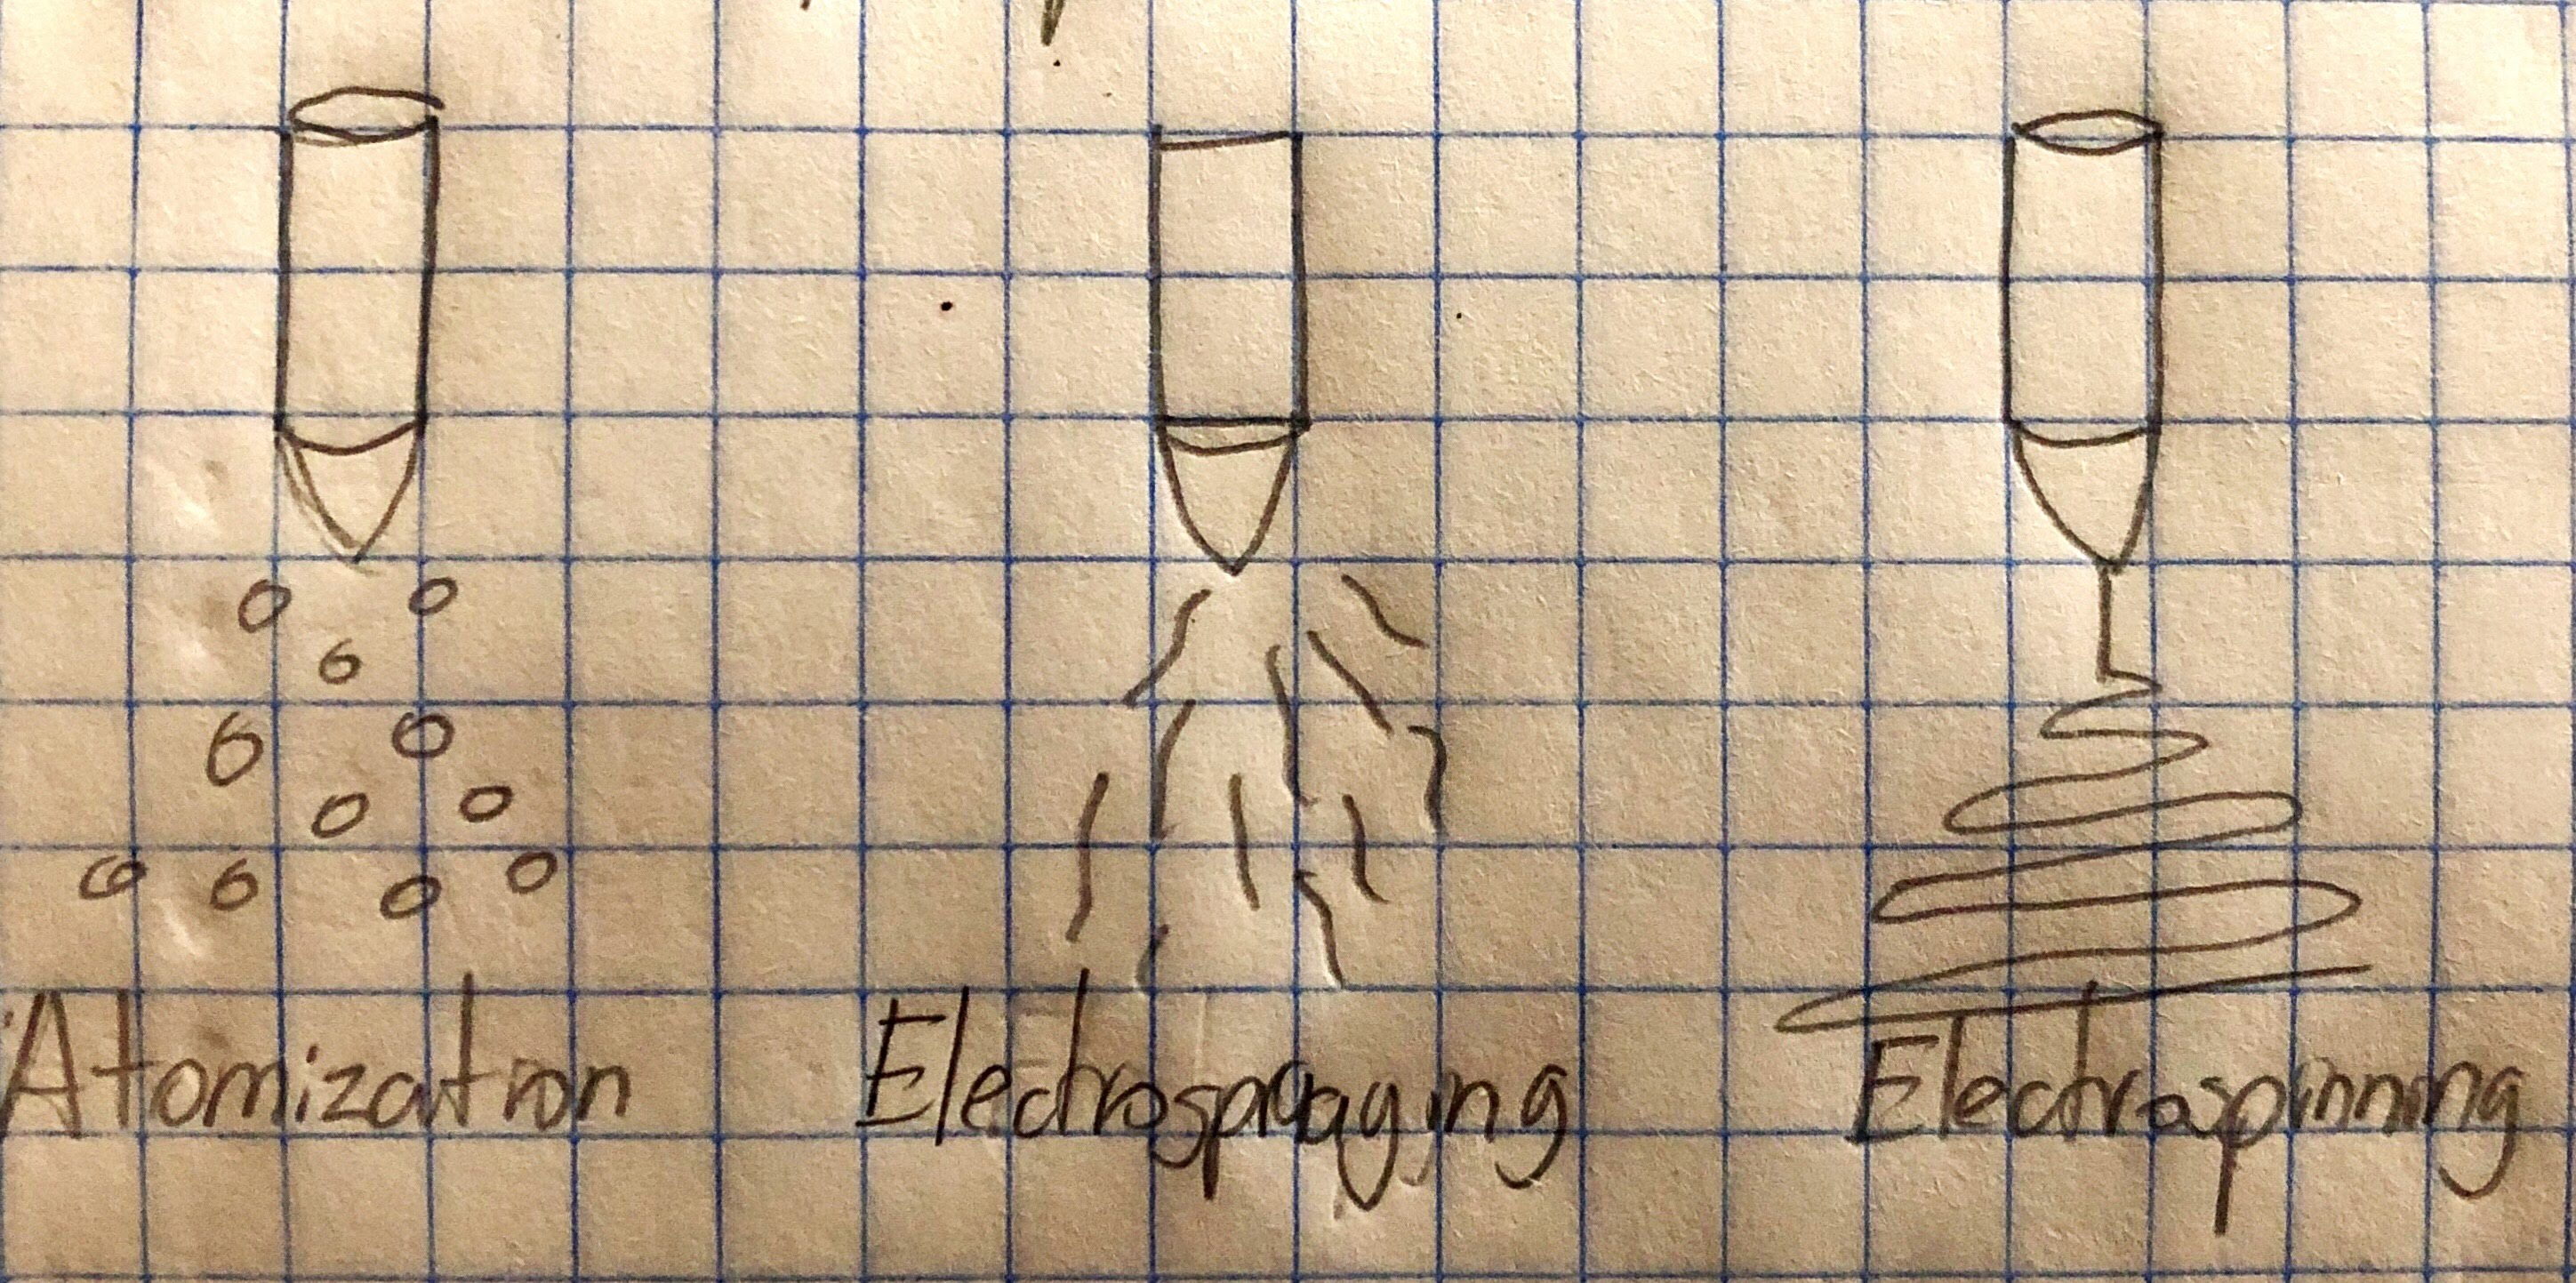
\includegraphics{images/f10bcbc9-719b-4a8d-8a38-930cc6ea2d0f-uimg_ehdprocesses.jpg}}{}
\makeatother 
\caption{{Electrohydro-dynamic techniques}}
\label{f-02e0e3cf88d6}
\end{figure}
\egroup




\subsection{Polymer reservoir: Polymer melt \& Polymer solution}Another electrospinning classification is the melt process. As Brown et al. \unskip~\cite{527120:13445499} discussed, the polymer melt is equivalent to the polymer solution electrospinning (in place of a polymer solution a melt is used). The use of a polymer melt increases the complexity of the process, because the nozzle syringe and spinneret required to be heated to maintain the polymer in a liquid state. The fibers produced in melt spinning are typically found to have larger diameters than those from the polymer solutions due to the higher viscosity of a polymer melt than its solution. The apparatus used by Brown et al. \unskip~\cite{527120:13445499} is depicted in .

[TODO: draw an apparatus used for melt electrospinning].

Despite the added complexity and thicker diameters, melt electrospinning  gets around the need to handle volatile solvents, making the process safer to be performed on larger scales, On the other hand, this technique gets rid of any solvent contamination.

The first report of a melt electrospun drug delivery system came from Nagy et al. \unskip~\cite{527120:13445555}, who prepared fibers by melt electrospinning of Eudragit EPO with carvedilol. The drug and polymer were melted and mixed to form a homogeneous solid mixture prior to spinning. The melt-spun fibers reached diameters of 5{\textendash}30 $\mu m $, compared to 300{\textendash}1000 $nm $ diameters produced from solution-spun fibers. 

This work has been built on to blend plasticisers with the polymer Eudragit EPO and carvedilol active ingredient.\unskip~\cite{527120:13445752} The plasticisers Triacetin, Tween 80 and Polyethylene Glycol were investigated by Attila et al. in order to reduce the melting point of the polymer-drug mixture. The temperature drop is desirable to minimize the occurring drug degradation.

Lian and Meng\unskip~\cite{527120:13445754} performed a comparison of poly(\ensuremath{\varepsilon }-caprolactone) (PCL) fibers fabricated by the melt and solution electrospinning techniques. Lian and Meng\unskip~\cite{527120:13445754} reported that melt spinning is preferable when the polymer presents a low solubility, on the other hand the melt fibers were produced in a slower release rate.  Lian and Men findings feature the solution-spun fibers to have a porous structure. Gernot et al.\unskip~\cite{527120:13534159} demonstrated that submicron-size fibers are possible through melt electrospinning. In their effort, they achieved a precise deposition of PCL fibers with diameters of $817 \pm 165 nm $. 

In literature, melt electrospinning has less evidence than the solution approach. However, melt electrospinning arises to be as flexible as its solution counterpart in handling multiple polymers, as reported in McCann's work\unskip~\cite{527120:13534572}. Currently, the melt electrospinning setup is harder to establish but the lack of research on this technique explains its unexplored potential.



\subsection{Dispensing nozzle}Coaxial electrospinning (co-electrospinning) requires de implementation of a dual needle nozzle, where one needle is nested concentrically inside another needle [TODO: draw nested needles]. \unskip~\cite{527120:13914792,527120:13914793} The purpose of the co-electrospinning setup is to produce core/shell fibers, unlike mono axial electrospinning that yields monolithic fibers. Sun et al. \unskip~\cite{527120:13914312} addressed electrospinning setups, where both the core and shell are comprised by PEO (poly(ethylene oxide)) and for a PEO shell with a poly(dode-cylthiophene) core. Sun et al. state that co-electrospinning has the potential to extend the range of materials that can be used for electrospinning. The shell solution can be modified to make the core solution spunable. It was also discovered that non-spunable solutions can by implemented as shell solutions in conjunction with a spunable core solution. \unskip~\cite{527120:13914968}

Some advantages that co-electrospinning setups can offer include the preempting the initial jet burst from the spinneret nozzle. On the other hand, as the morphology and shape of the fibers depend on the polymer solution properties, the use of a co-axial nozzle allows the amendment of the material properties by producing bubbles, scaffolds and particles. \unskip~\cite{527120:13914748,527120:13914750}. As in conventional NFES, in co-electrospinning, the needle tip is connected to a high voltage power supply with a grounded collector. With the influence of high electric fields, the fibers are prone to brake into separate layers due to the whipping instabilities as the jet travels to the substrate. The instability can be mitigated by adding additional ring electrodes between the spinneret and the grounded collector. \unskip~\cite{527120:13915304}



\subsection{Stretching forces}



\subsubsection{Electric Field}Electrospinning (electrostatic fiber spinning) is a fiber fabrication approach that implements an electric field produce fibers by an electrical potential difference between the syringe needle and the collector. The typical electrospinning setup applies an electrostatic charge to the polymer fluid at the tip of the needle nozzle, which results in the formation of the Taylor cone \unskip~\cite{527120:13659828}, from which a single polymer jet is ejected to the grounded collector. From the Taylor cone, the supplied polymer jet (typically a polymer solution) accelerates and reduces in diameter. The fiber finally develops with the complete solvent evaporation. Electrospun fibers are prone to splitting with the increase in acceleration, where multiple fibers are yield in a process known as electrospraying \unskip~\cite{527120:13659925}.

The electrospinning process starts with charging a polymer solution droplet. When a polymer solution is administrated with a syringe pump, solution droplets will fall under the influence of gravity. The solution dripping stops when the electric field is strong enough to break the solution's surface tension, causing the droplet to change shape forming a polymer solution jet\unskip~\cite{527120:12033655}.

Shin et al. \unskip~\cite{527120:13659926} reported that the growth of the whipping instability is one important element within the electrospinning technique. As detailed in Shin's work, weak electric fields produce a single uniformly thinning jet, and strong electric fields the jet becomes unstable after traveling a short distance.



\paragraph{High voltage power supply: Direct Current \& Alternating Current}Direct current (DC) is typically used in electrospinning with the electrons flowing in one direction. Alternate current (AC) implementations are also studied as the AC creates a change in the direction of the current flow. Kessick et al.\unskip~\cite{527120:13444381} demonstrated the implementation of AC power supplies in the production of polymer fibers.

The AC electrospinning setup is similar to that for the DC variant. AC electrospinning apparatus do not require a grounded collector as the current alternates. In AC, the produced fibers are prone to carry an electric charge, while those generated shortly after have an opposite charge. The difference in charges lead the fibers to discharge on each other, creating an aerogel plume of fibers. The optimal AC frequency depends on the materials used and is typically within of 50 $Hz $ {\textendash} 1 $kHz $. \unskip~\cite{527120:13443405}

The AC technique has been studied for drug loaded related applications. Balogh et al. \unskip~\cite{527120:13445177} compared fibers fabricated by DC and AC spinning techniques. They produced fibers by using three polymers: Eudragit EPO (cationic copolymer), Eudragit L100-55 (anionic polymer) and poly(vinyl pyrrolidone) (PVP) (neutral polymer). Balogh et al. discovered AC and DC electrospinning can produce fibers with all three polymers. However, The AC process allowed the implementation of faster flow rates than in the DC setup. The DC electrospinning technique generated fibers with a maximum flow rate of 5 $ml/h $; on the other hand, the AC setup allowed an increase in flow rate up to 40 $ml/h $. AC electrospinning approach is as effective as the DC technique in producing drug delivery systems.



\subsubsection{Centrifugal force}The spinning processes require the implementation of a force to break the polymer source into a polymer jet. Centrifugal spinning intends to produce fibers by the use of a rotating polymer source. The centrifugal force generated from typical rotatory speeds above 2000 rpm, results in fiber formation. \unskip~\cite{527120:13535559,527120:13535561}.

The centrifugal force technique is applied to polymer solutions and melts. This approach is used in applications were the precise deposition of the fibers is not relevant and production rate is to be maximized \unskip~\cite{527120:13535894}.  Efforts in centrifugal spinning are focused on drug delivery applications. Zander \unskip~\cite{527120:13535977} fabricated polycaprolactone (PCL) fibers using the solution and melt variants of the centrifugal approach. Zander's fibers were produced with rotatory speed between three and 18 thousand revolutions per minute with $10 \mu m $ in diameter. 

On the other hand, PCL and PVP fibers were generated by Amalorpava et al. \unskip~\cite{527120:13536089}.  Amalorpava achieved sub micron/size fiber diameters for drug release purposes and bacteria growth inhibition properties. Literature\unskip~\cite{527120:13536446} has shown that centrifugal approach has a simple setup that promises a large scale fabrication of fibers.

In some cases the centrifugal force implementations and pressurized gyration can be combined with an electric field. The implementation of two stretching forces (centrifugal and electrical forces), can help solvent evaporation\unskip~\cite{527120:13536560}. Centrifugal electrospinning implements the same setup as the standard centrifugal spinning with the addition of a high voltage power supply between the rotating dispensing nozzle and the collector. The combined method has evidence to yield parallel fibers\unskip~\cite{527120:13536841,527120:13536900,527120:13537392,527120:13537393} at a higher rate \unskip~\cite{527120:13536841,527120:13536900} than the standard electrospinning approach.



\subsubsection{Blowing forces}Nano fibers can be produced with the implementation of pressurized gas with a polymer solution. The setup used for blow spinning is similar to the one used in standard electrospinning, where the polymer precursor is dispensed at a controlled rate. Unlike traditional electrospinning, in the solution blow spinning setup the needle nozzle applies pressurized gas to the polymer solution through an outer spinneret\unskip~\cite{527120:13538056}. 

[TODO: draw an apparatus used for solution blow spinning or melt blowing] \unskip~\cite{527120:13538056}.

Poly(lactic acid) (PLA) fibers have been produced by solution blow spinning. Oliveira et al. \unskip~\cite{527120:13539278} fabricated the fibers from $6 wt\% $ PLA solutions with progesterone for live stock reproductive cycle regulation applications. On the other hand, Souza et al.\unskip~\cite{527120:13538056} conducted a study to compare the standard electrospinning and the solution blow spinning techniques. Poly(3-hydroxybutyrate-co-3-hydroxyvalerate) were fabricated by both methods. The fibers produced by electrospinning had thicker diameters and their size uniformity was higher in the fibers produced by solution blow spinning.

Jiang et al.\unskip~\cite{527120:13554126} combined the blowing technique with the electrospinning approach. The blow electrospinning technique implements both electric and gas flow forces to stretch the fibers. Jiang used an apparatus similar to those used in traditional electrospinning. The experimental setup requires a coaxial needle nozzle with a pressurized gas flow along with a potential difference between the dispensing needle and the grounded collector. 

[TODO: draw Figure apparatus used for solution blow spinning or melt blowing]



\subsubsection{Mechanical force}Mechanical drawing comprises the simple technique to produce fibers by stretching the polymer solution with a glass pipette. \unskip~\cite{527120:14024998} Nevertheless, the drawing technique is not scalable or with practical applications. \unskip~\cite{527120:14025041} Touch-spinning methods have been developed to introduce a scalable technique for the production of nano fibers. Touch-spinning comprises a rotating stage with an embedded glass rod. [TODO: draw touch spinning setup]. Where a polymer solution is supplied from a syringe needle such that the tip of the glass rod makes contact with the polymer solution as it rotates, creating fibers. The rotation stretches the fiber, causing the fiber to increase in length and decrease in diameter. The increase in length causes the fiber surface are to increase and therefore making the polymer solution solvent to volatilize, ending with a dry fiber within the collector.

The touch spinning technique implies that the fiber diameter can be controlled by the rotation speed and the polymer solution concentration. The main difference relays on the fact that the touch spinning method implements mechanical control to manipulate and stretch the fibers during the fabrication process, guiding the fiber in the collector enabling better control over fiber alignment.\unskip~\cite{527120:14091959}



\subsubsection{Microfluidic forces}The microfluidic spinning technique manipulates and controls the polymer solution in networks of micrometer channels. The channel network are typically embedded in a microfluidic chip, where the solution deposition rate is controlled by active components (pumps and valves) with a computer. Cheng et al. \unskip~\cite{527120:13656236} compared and combined the microfluidic spinning and electrospinning techniques. 

On the other hand, Kang et al. \unskip~\cite{527120:13656548} managed to fabricate micro fibers by imitating the "silk spinning" process of spiders. Kang's micro fibers properties were modified using a microfluidic system with a programmable flow control. The current microfluidic spinning approach is not scalable to a large fiber production, however it enables the fabrication of high-complex fibers that are not easily achieved by other methods.

[TODO: draw Figure apparatus used for microfluidic spinning]

Microfluidic techniques offer the possibility to embed several components into a single fiber, where each component can be released at different parts of the fiber. 



\subsection{Nozzle-to-substrate distance}[TODO: draw FFES setup], depicts the typical setup for the conventional far-field electrospinning (FFES). As stated in previous sections, the precursor polymer droplet becomes charged with the employment of an electric field between the polymer solution and the collector\unskip~\cite{527120:14135125}. When the polymer solution surface tension is overcome by the electric field potential difference a jet is formed, starting the electrospinning process. The electrospinning process can be break down into two steps: i) first the jet travels in a straight line, and ii) the jet begins to curl due to bending and whipping instabilities \unskip~\cite{527120:13444381,527120:14135543}. The fiber spatial control in far-field electrospinning is limited due to the instabilities, inhibiting the precise deposition of fibers.

In the intent to achieve controlled fiber deposition, Sun et al. \unskip~\cite{527120:11974321} reported an electrospinning variation known as near-field electrospinning (NFES). [TODO: draw NFES setup], describes the near-field electrospinning setup, where the distance between the dispensing nozzle and the collector is reduced to write fibers while the jet travels in a straight line. Moreover, some mechanical influence is required to deposit fibers precisely. The mechanical force is introduced by moving collector. If the polymer solution jet speed is faster than the speed of the moving collector, the written fiber will curl; on the other hand, if the collector moves faster than the polymer jet, the fiber will gradually diminish \unskip~\cite{527120:11974327,527120:11974326}. Currently, due to the lack of theoretical models, the near-field electrospinning process parameters (such as the collector speed) are typically tuned by experience and experimentation only.

The main difference between NFES and FFES is the distance between the needle and the collector which is higher in FFES (about 10 cm) compared to NFES which ranges in the mm scale. The short distance allow the production of well aligned fibers within particular designs. [7]


\bgroup
\fixFloatSize{images/461590fc-21b9-4974-88ef-bdfb00006f73-udrf_nfes.jpg}
\begin{figure}[!htbp]
\centering \makeatletter\IfFileExists{images/461590fc-21b9-4974-88ef-bdfb00006f73-udrf_nfes.jpg}{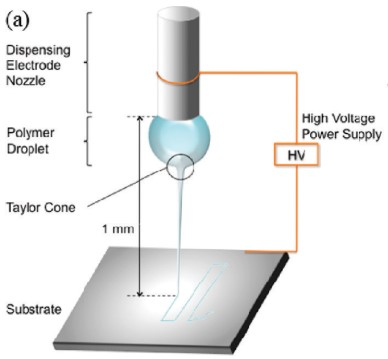
\includegraphics{images/461590fc-21b9-4974-88ef-bdfb00006f73-udrf_nfes.jpg}}{}
\makeatother 
\caption{{Typical near-field electrospinning set-up \unskip~\protect\cite{527120:11973130}.}}
\label{f-8e5a75d9ba17}
\end{figure}
\egroup

    
\section{Properties that Improve Accuracy of Nano-Fiber Deposition}
Near-field electrospinning is considered to be an outstanding technique to fabricate polymer fibers with spatial control and it has suffered several modifications to improve the precision and accuracy of the fiber deposition. This paper intents to collect the NFES variants of electrospunable polymer solutions with spatial control in recent research.



\subsection{Low-Voltage NFES (LV NFES) \unskip~\protect\cite{527120:11973130}}Some differences have been discovered between LV-NFES and conventional NFES. Low voltage near field electrospinning produces thinner fibers with lower voltages. Moreover, when implementing a moving stage, the fibers are affected by the mechanical stretching. Bisht et al. \unskip~\cite{527120:11973130} reported that thinner diameters are yield with the increase of the x-y stage velocity, and larger diameters by decreasing the stage velocity.

-{\textgreater} A continuous method for controlled electrospinning of polymeric nano fibers on two-dimensional (2D) and three-dimensional (3D) substrates using low voltage near-field electrospinning (LV NFES). The method overcomes some of the drawbacks in more conventional near-field electrospinning by using a super elastic polymer ink formulation. The visco-elastic nature of our polymer ink enables continuous electrospinning at a very low voltage of 200 V, almost an order of magnitude lower than conventional NFES, thereby reducing bending instabilities and increasing control of the resulting polymer jet. In one application, polymeric nano fibers are freely suspended between micro structures of 3D carbon on Si substrates to illustrate wiring together 3D components in any desired pattern.{\textless}-



\subsection{Scanning Tip Electrospinning \unskip~\protect\cite{527120:11974306}}-{\textgreater} A continuous near-field electrospinning (NFES) process has been developed to deposit solid nano fibers with orderly patterns over large areas. Before the onset of electrospinning, a bias voltage is applied to a semi-spherical shaped polymer droplet outside of a syringe needle, and a probe tip mechanically draws a single fiber from the droplet to initiate continuous NFES. Contrary to the conventional electrospinning process, we show that decreasing electrical field in continuous NFES results in smaller line width deposition, and nano fibers can be assembled into controlled complex patterns such as circular shapes and grid arrays on large and flat areas. {\textless}-



\subsection{3D Electrospinning \unskip~\protect\cite{527120:11974313} \mbox{}\protect\newline Electrohydro-dynamic 3D Print-patterning or Electrohydro-dynamic Jetting \unskip~\protect\cite{527120:11974310}}-{\textgreater} Characterized the behavior of polymer jet from near-field electrospinning onto the ink-jet patterned paper with conductive Ag nano particles in order to form the controlled three-dimensional nano structures. Using ink-jet patterned paper with conductive ink as a collector, the polymer jet is induced to the pre patterned shape through the concentrated electric field caused by singularity between the spinneret and the printed patterns. Due to the electric field enhancement of the deposited electrospun fiber, an additionally spun fiber can be stacked on the deposited fibers directly. Therefore, the controlled three-dimensional nano/micro structures can be successfully realized by the proposed method. We characterized the deposition of the electrospun fiber according to the distance between the ink-jet printed pattern and the spinneret. In addition, the sharp edged three-dimensional micro-structures were fabricated by carrying out the electrospinning on the patterns with various angled edges. A CCD camera was used to observe the behavior of the polymer jet, and the SEM image was analyzed to confirm that the fibers are stacked as desired.

Uncover a new method for the preparation of bio-polymer scaffolds and demonstrate its potential for the development of organs with the aid of tissue engineering. Two novel nano-composite polymers, a non-biodegradable polyhedral oligomeric silsesquioxane-poly (carbonate-urea)urethane and a biodegradable polyhedral oligomeric silsesquioxane-polycaprolactone-poly(carbonate-urea)urethane, have been subjected to flow in an electric field. Electrically forced micro-threading of the polymers occurs and a three-dimensional print-patterning device was used to deposit fine (⬍50 \ensuremath{\mu}m) threads of polymer according to a pre-designed architecture to prepare scaffolds. The technique can offer tremendous potential in the development of organs. {\textless}-



\subsection{Multinozzle NFES \unskip~\protect\cite{527120:11974322,527120:11974323,527120:11974324}}-{\textgreater} Multinozzle electrospinning systems are designed to increase productivity, while near-field electrospinning (NFES) systems are designed to deposit solid nano fibers in a direct, continuous, and controllable manner. In this paper, several multinozzle NFES setups are tested. The experiment reveals that the deposition distance becomes larger when working distance and needle spacing increase, and the influence of voltage is relatively weaker. The deposition of double nozzle NFES has been studied with Coulomb's law and theoretical derivation has been verified by the experimental conclusion. The experiment result and theoretical derivation are helpful to get different distance of direct-written fibers by adjusting working distance or needle spacing to change distance of fibers largely and adjusting voltage to change distance slowly. Through these efforts, it is convenient to adjust the distance of straight fibers in multinozzle system. [1]

For large area micro/nano pattern printing, multi-nozzle electrohydrodynamic (EHD) printing setup is an efficient method to boost productivity in near-field electrospinning (NFES) process. And controlling EHD multi-jet accurate deposition under the interaction of nozzles and other parameters are crucial concerns during the process. The influence and sensitivity of various parameters such as the needle length, needle spacing, electrode-to-collector distance, voltage etc. on the direct-write patterning performance was investigated by orthogonal experiments with dual-nozzle NFES setup, and then the deposition distance estimated based on a novel model was com- pared with measurement results and proven. More controllable deposition distance and much denser of aligned nano fiber can be achieved by rotating the dual-nozzle setup. This study can be greatly contributed to estimate the deposition distance and helpful to guide the multi-nozzle NFES process to accurate direct-write pattern in manufacturing process in the future.

To mass-volume fabricate micro- and nano scales aligned pattern, multi-nozzle near- field electrospinning (NFES) direct-writing technology is well proposed as a high- efficiency method in electrohydrodynamic (EHD) printing process. However, the interference effect among adjacent nozzles and coupling effect of various parameters have restricted to investigate deposition characteristic of multi-nozzle NFES and control EHD multi-jet deposition accuracy. In order to improve the accuracy of EHD multi-jet deposition with high-efficiency printing process, the experimental result compared with theoretical method were discussed. In this work, the influence of multi-nozzle geometry distribution and electrospinning parameters on deposition characteristic was studied with multi-nozzle NFES setup, and nozzles were in linear array. The deposition distance and homogeneity of aligned nano fibers were measured and explained with coefficient of dispersion on electric field among nozzles by simulation. Moreover, deposition distance of multi-nozzle NFES process was evalu- ated by modified theoretical derivation based on our previous studies. The modified theoretical derivation showed a good agreement with experiment results, and indicated that multi-nozzle NFES could accurately and efficiently direct-write aligned array pattern in the future. {\textless}-



\subsection{Electrohydro-dynamic Writing or Mechanoelectrospinning (MES) \unskip~\protect\cite{527120:11974311} \mbox{}\protect\newline Electrohydro-dynamic Direct-Write (EDW) \unskip~\protect\cite{527120:11974328}}-{\textgreater} Direct writing of hierarchical micro/nano fibers have recently gained popularity in flexible/stretchable electronics due to its low cost, simple process and high throughput. A kinetically controlled mechanoelectrospinning (MES) is developed to directly write diversified hierarchical micro/nano fibers in a continuous and programmable manner. Unlike conventional near-field electrospinning, our MES method introduces a mechanical drawing force, to simultaneously enhance the positioning accuracy and morphology controllability. The MES is predominantly controlled by the substrate speed, the nozzle-to-substrate distance, and the applied voltage. As a demonstration, smooth straight, serpentine, self-similar, and bead-on-string structures are direct-written on silicon/elastomer substrates with a resolution of 200 nm. It is believed that MES can promote the low-cost, high precision fabrication of flexible/stretchable electronics or enable the direct writing of the sacrificial structures for nano scale lithography.

AC pulse-modulated electrohydrodynamic direct-writing (EDW) was utilized to direct-write orderly micro/nano fibrous structure on the flexible insulating polyethylene terephthalate (PET) substrate. During the EDW process, AC electrical field induced charges to reciprocate along the jet and decreased the charge repulsive force that applied on charged jet. Thanks to the smaller charge repulsive force, stable straight jet can be built up to direct-write orderly micro/nano fibrous structures on the insulating substrate. The minimum motion velocity required to direct-write straight line fibrous structure on insulating PET substrate was 700 mm/s. Moreover, the influences of AC voltage amplitude, frequency, and duty cycle ratio on the line width of fibrous structures were investigated. This work proposes a novel solution to overcome the inherent charge repulsion emerging on the insulating substrate, and promotes the application of EDW technology on the flexible electronics. [1]. {\textless}-



\subsection{Mechano-Electrospinning \unskip~\protect\cite{527120:11974304}}-{\textgreater} A mechano-electrospinning method is presented to direct-write oriented nano fiber with high deposition accuracy in continuously tunable manner. This method uses a large nozzle to deposit high-resolution fiber-arrays by near-field localization. Due to the existence of mechanical drawing force, a higher resolution pattern can be direct-written by a lower voltage, which just keeps the Taylor cone stable. Then the fiber is stretched through a moving substrate, by which the deposited fiber can be continuously tuned from 400nm to 200nm in a linear relation- ship. The effects of the speed on the diameter and morphology of fibers are studied, and the analysis of the mechanism of the fiber alignment is given. The positionability and controllability make mechano-electrospinning very different from the traditional electrospinning, which only collects the fibers in the form of nonwoven fabric. In addition, the fibers fabricated by this method can directly deposit over a large flat area in the form of arrays and complex patterns with high precision. {\textless}-



\subsection{Suspension NFES \unskip~\protect\cite{527120:12033656}}-{\textgreater} Near-field electrospinning (NFES) is widely recognized as a versatile nano fabrication method, one suitable for applications in tissue engineering. Rapid developments in this field have given rise to layered nano fibrous scaffolds. However, this electrostatic fabrication process is limited by the electric field inhibitory effects of polymer deposition. This leads to a major challenge: how to surpass this limitation on planar/layered constructs. While the current focus in this area largely lies with the investigation of new materials, techniques and increasing precision of NFES systems and patterning, exploration of complex collector substrates is often restricted by (i) available technology and (ii) access to complex electrode manufacturing tools. To achieve nano fiber arrays suspended in free space, this paper documents both the development of an integrated NFES system and the potential of standing electrodes manufactured via selective laser melting. This system was first tested by 2D patterning on planar silicon, using polyethylene oxide polymer solution. To demonstrate suspension NFES, two patterns operating within and around the standing electrodes produced high volume suspended nano arrays. Image analysis of the arrays allowed for the assessment of fiber directionality and isotropy. By scanning electron microscopy, it was found that a mean fiber diameter of 310 nm of the arrays was achieved. Effectively maneuvering between the electrode pillars required a precision automated system (unavailable off-the-shelf), developed in-house. This technique can be applied to the fabrication of nano fiber structures of sufficient volume for tissue engineering. {\textless}-



\subsection{Helix Electrohydro-dynamic Printing (HE-printing) \unskip~\protect\cite{527120:11974308} \mbox{}\protect\newline Electrohydro-dynamic (EHD) jet printing \unskip~\protect\cite{527120:11974320}}-{\textgreater} Micro/nano serpentine structures have widespread applications in flexible/stretchable electronics; however, challenges still exist for low-cost, high-efficiency and controllable manufacturing. Helix electrohydrodynamic printing (HE-printing) has been proposed here to realize controllable direct-writing of large area, highly aligned serpentine micro/nano fibers by introducing the rope coiling effect into printing process. By manipulating the flying trajectory and solidification degree of the micro/nano jet, the solidified micro/nano fiber flying in a stabilized helical manner and versatile serpentine structures deposited on a moving collector have been achieved. Systematic experiments and theoretical analysis were conducted to study the transformation behavior and the size changing rules for various deposited micro structures, and highly aligned serpentine microfibers were directly written by controlling the applied voltage, nozzle-to-collector distance and collector velocity. Furthermore, a hyper-stretchable piezoelectric device that can detect stretching, bending and pressure has been successfully fabricated using the printed serpentine micro/nano fibers, demonstrating the potential of HE-printing in stretchable electronics manufacturing.

Electrohydrodynamic (EHD) jet printing is a direct-writing technique which ejects ink through a fine noz- zle using an electric field, which has the advantages of high-resolution, rapid printing speed and a wide range of ink selectivity. In this article, the EHD jet printing system is utilized to print patterns of polystyrene (PS) nano fibers. The effect of parameters such as ink concentration, working distance, applied voltage, and stage speed on the diameter of the printed nano fibers was investigated. The EHD jet printing technology is further utilized to print various patterns of polydiacetylene (PDA)-embedded PS nano fibers. The EHD jet printing based nano fiber printing is advantageous over conventional electrospining based approaches in terms of patterned PDA images. In addition, an advanced EHD jet printing system which is adopted for aligned nano fiber printing will expand the application of nano fibers from bio and chemical sensors to tissue engineering and electronics. {\textless}-



\subsection{Airflow-assisted Electrohydro-dynamic Direct-writing (EDW) \unskip~\protect\cite{527120:11974312}}-{\textgreater} Electrohydrodynamic direct-writing (EDW) is a developing technology for high-resolution printing. How to decrease the line width and improve the deposition accuracy of direct-written patterns has been the key to the promotion for the further application of EDW. In this paper, an airflow-assisted spinneret for electrohydrodynamic direct-writing was designed. An assisted laminar airflow was introduced to the EDW process, which provided an additional stretching and constraining force on the jet to reduce the surrounding interference and enhance jet stability. The flow field and the electric field around the spinneret were simulated to direct the structure design of the airflow-assisted spinneret. Then, a series of experiments were conducted, and the results verified the spinneret design and demonstrated a stable ejection of jet in the EDW process. With assisted airflow, the uniformity of printed patterns and the deposition position accuracy of a charged jet can be improved. Complex patterns with positioning errors of less than 5\% have been printed and characterized, which provide an effective way to promote the integration of micro/nano systems. {\textless}-



\subsection{Tethered Pyro-Electrohydro-dynamic Spinning (TPES) \unskip~\protect\cite{527120:11974307}}-{\textgreater} Although electrospinning (ES) allows the production of unsurpassed nano scale polymer fibers, the major draw- \mbox{}\protect\newline backs are the nozzle-clogging and single-jet spinneret, respectively. This is a real limitation in terms of usable polymers and for patterning active organics. Nowadays the micro-engineering of smart materials could represent a new route for many fields of technology ranging from the production of electronic and photonic devices [1\ensuremath{-}3] to regenerative medicine and tissue engineering. [4\ensuremath{-}7] An enormous technological interest is related to the possibility of patterning fibers directly in well-ordered patterns avoiding the deposition of nonwoven sub micrometer mats often occurring in ES. [8,9] In the past decade several attempts have been made using field- induced [10\ensuremath{-}13] and near-field ES, [14,15] but only very recently, with the introduction of mechano ES, [16] has the production of well- ordered fiber patterns been achieved. Nevertheless, some drawbacks related to the complexity of the setup, the operating temperature, and the selection of usable materials for problems related to nozzle clogging still persist. Moreover, high temperature can cause deterioration of the optical and electronic properties of active organic materials eventually embedded in the functionalize [d fibers. On the other side, interfering effects due to closeness of multiple electrified nozzles ban working with multiple spinnerets. Here we introduce a revolutionary nozzle-free approach, the tethered pyro-electrodynamic spinning (TPES) operating in wireless modality, i.e., without electric circuit, electrodes, and voltage supply. This novel approach definitively simplifies the ES apparatus extending the nano fiber spinning also to active organic polymers preserving at the same time all the properties of conventional systems. Fiber drawing from the liquid polymer is driven through the pyroelectric charge generated into a ferro-electric crystal (i.e., LiNbO3) able to induce the electro- hydrodynamics (EHD) pressure required for polymer manipulation without wires. The approach is highly flexible, simple, compact, and cost-effective when compared with classical ES, and last but not least, it allows working safely, avoiding the use of high-voltage equipment at kV scale. For the first time, in site observation of fiber drawing is provided allowing real-time adjustments and full control of the process. Moreover, the TPES adds to the capabilities of conventional ES the chance of printing polymer fibers even in the case of multiple drops opening the way to the multi jetting spinneret modality for multiplexing and speeding up the fabrication process. Printing of micro- and nano fibers directly from a polymer drop with unprecedented order, direct writing of sharp/straight edges, and easy multi jets electrospinning are demonstrated and reported. Experimental fabrication of patterns embedded with active molecules ensures that functionalized patterns preserve their functionalities after the TPES process. Results regarding the use of smart patterns for keeping alive and viable cultured cells are discussed. This study opens the way to innovative optogenesys analysis, guiding light for generating or trans- porting optical/electronic signals from and to cells. [17\ensuremath{-}21] The setup proposed in this work, unlike the conventional ES, is electrode-free and nozzle-free {\textless}-
    
\section{Polymer Solution}
In electrospinning, it is typically agreed that the diameter of the fibers increased with higher concentration due to greater viscosity which withstands stretching. In near field electrospinning, similar observations have been reported where concentration increases, fiber diameter increased\unskip~\cite{527120:11974306,527120:11974329}. However, in separate studies by Pan et al.\unskip~\cite{527120:11974317,527120:12321129} using poly(\ensuremath{\gamma }-benzyl \ensuremath{\alpha }, l-glutamate) and polyvinylidene fluoride (PVDF) reported reduction in fiber diameter with increasing concentration.
\begin{table}[!htbp]
\caption{{Approximation process to estimate the critical polymer concentration. Several polymer concentrations are tried and the resulting jets are observed until a continuous stream is achieved.} }
\label{tw-8687dd17082c}
\def\arraystretch{1}
\ignorespaces 
\centering 
\begin{tabulary}{\linewidth}{LL}
\tbltoprule Observation & Concentration Adjustement\\
\tblmidrule 
Dripping, no stream &
  Increase\\
Splitting small droplets &
  Increase slightly\\
Steady stream &
  No concentration adjustment\\
Splitting large globs &
  Decrease slightly\\
Nozzle clogging  &
  Decrease\\
\tblbottomrule 
\end{tabulary}\par 
\end{table}




\subsection{Polymers}The polymer selection is in function on the intended application. For example, a fast dissolving hydrophilic polymer such as poly(ethylene oxide) (PEO) is used for fast drug delivery systems. Otherwise, slow dissolving polymers such as poly($\varepsilon $-caprolactone) (PCL) or poly(lactic-co-glycolic acid) (PLGA) are implemented. \unskip~\cite{527120:13082763}

The polymer molecular weight along with the polymer concentration and solvent selection have a direct effect on the solution viscosity, conductivity and surface tension, hence the solution behavior in the electrospinning process. The spunable viscosity range varies with the polymer and solvent. 

Solutions with low viscosity are prone to insufficient polymer chain entanglements to produce fibers.\unskip~\cite{527120:13082763} On the other hand, if the solution is too viscous, then the surface tension cannot easily be overcome by the electric field. In both cases, the result can be droplets or particles forming rather than fibers; see Table~\ref{tw-8687dd17082c}.



\subsection{Solvents}The solvent used must be capable of dissolving the polymer of interest at an appropriate concentration to form fibers, and must posses a suitable volatility. A low-volatility solvent like water may fail to evaporate completely over the distance between the spinneret and the collector. When the fibers form, they will hence contain residual water owing to this incomplete evaporation. The residue solvent will subsequently evaporate from the fibers upon storage, resulting in ribbon-like (flattened) fibers, wrinkles on the fiber surface or fused fibers. On the other hand, a high-volatility solvent may evaporate very quickly, leading to larger fiber diameters (less time for elongation before solidification) and clogging of the spinneret (due to drying of the liquid at the spinneret before jetting, or drying of the Taylor cone during jetting). Solvents commonly used for electrospinning include ethanol, chloroform, dichloromethane and hexafluoroisopropanol.

Mixtures of miscible solvents can be used to ensure that sufficient polymer can be dissolved to give a solution of appropriate viscosity and volatility with suitable dielectric constant range to allow fiber formation. However, care must be taken because using a mixture of solvents with very different volatilities can result in porous fiber structures, as reported by Katsogiannis et al. for organic solvent mixtures with dimethyl sulfoxide (DMSO).\unskip~\cite{527120:13082766} DMSO evaporates much more slowly than the organic solvents used, which results in its incorporation into the fibers. The DMSO will eventually evaporate, yielding porous fibers.

It is also important to take into account the surface tension of the solution. Solvents with very high surface tensions (e.g. water) can result in instability arising during the spinning process, and a broad range of fiber diameters in the products. If necessary, a surfactant can be added to reduce the surface tension, but this will be incorporated into the fibers produced.
    
\section{Effect of the NFES Parameters}

\bgroup
\fixFloatSize{images/d29b646e-eca6-4b31-ab15-4cfc6fc94809-udrf_electrospinningvariants.jpg}
\begin{figure*}[!htbp]
\centering \makeatletter\IfFileExists{images/d29b646e-eca6-4b31-ab15-4cfc6fc94809-udrf_electrospinningvariants.jpg}{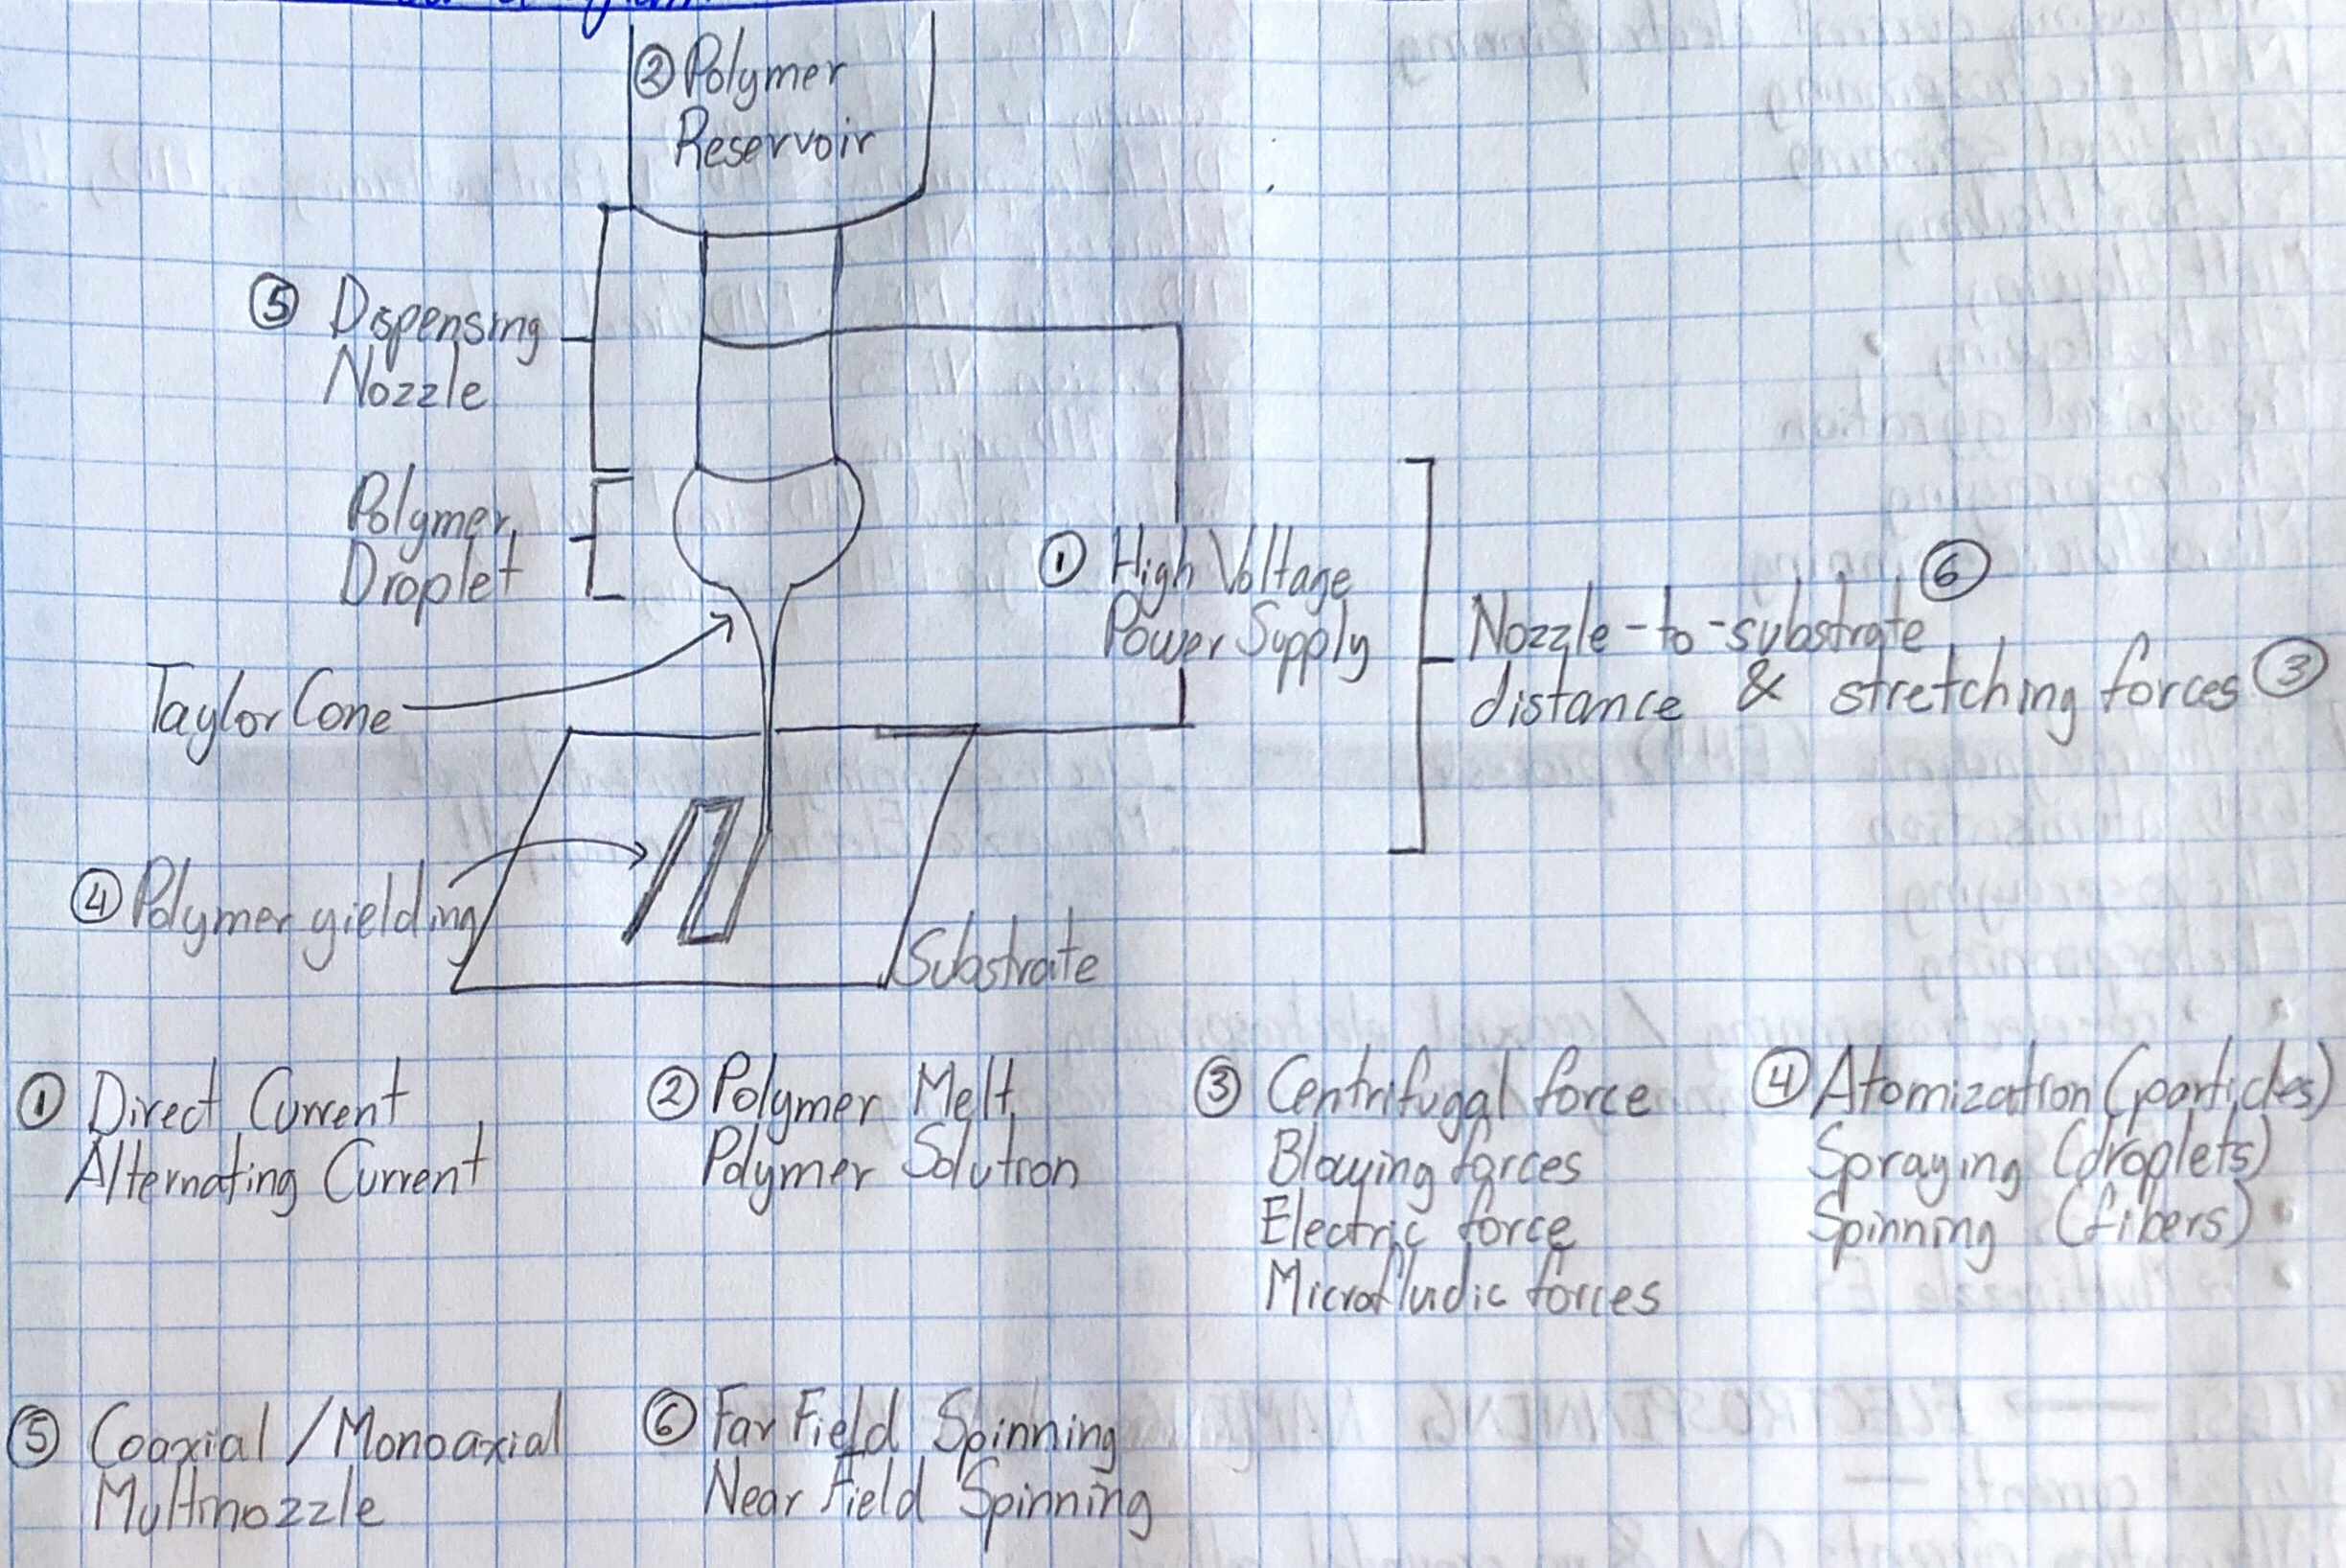
\includegraphics{images/d29b646e-eca6-4b31-ab15-4cfc6fc94809-udrf_electrospinningvariants.jpg}}{}
\makeatother 
\caption{{Near-Field ES Process Parameters}}
\label{f-3629d3a3f9cf}
\end{figure*}
\egroup
To spin nano fibers at close distances, the initial diameter of the jet is required to be as small as possible since stretching of the thread is limited. Kameoka et al.\unskip~\cite{527120:12321556} demonstrated that a small initial spinning radius can be achieved using an atomic force microscope tip with a small polymer solution drop at the tip.

Near-field electrospinning, has exhibited to be capable fabricate nano fibers over and nano fiber patterns \unskip~\cite{527120:11974321}. Nevertheless, having a small polymer solution drop at the nozzle tip limits the length of the fibers that can be fabricated in a continuous manner. Using a spinneret with a reservoir (e.g. syringe) of solution generally produces fibers with diameter of a few micrometers \unskip~\cite{527120:11974310,527120:11974326}, since it creates a limit to which the nozzle inner diameter can be reduced to allow the solution to flow through.

Coppola et al.\unskip~\cite{527120:11974307} have showed a NFES variant that allows polymer nano fibers to be deposited directly from a polymer drop, averting the issue of nozzle clogging. The fibers are also prone soaking after deposition thus giving the fibers a semi-circular cross-section as depicted in Xue et al.'s\unskip~\cite{527120:11974326} work. 



\subsection{Nozzle spinneret}The thinnest nozzles in literature so far are about 100 $\mu m $ in diameter, for instance Chang et al.\unskip~\cite{527120:11974306} used a 100 $\mu m $ inner diameter needle tip to electrospin poly(ethylene oxide) (PEO) and Camillo et al.\unskip~\cite{527120:12322072} used a micro-diameter tip Tungsten spinneret in a 26G needle to electrospin co-polymer, poly[2-methoxy-5-(2-ethylhexyloxy)-1,4-phenylenevinylene] (MEH-PPV) with poly(ethylene oxide) (PEO). The nozzle most commonly comprises a simple narrow-bore, blunt-end metal needle. The diameter of the needle can vary, but most commonly researches work with internal diameters below 1 $mm $ . This translates to needles of gauge 18{\textendash}22. In general, this simple spinneret design can be used to achieve successful spinning. A blunt-end rather than a tapered-end for the needle exit is important as the size distribution of the products increase with an increase in needle tip angle. However, it should be noted that there will be some interactions between the solvent and polymer molecules in the solution and the metal surface of the spinneret. There will exist some attractive forces between the polar groups in the polymer and the electro positive metal surface, which can act counter to the drawing force of the electric field and can pull the polymer solution back into the spinneret. It has been found that coating the spinneret exterior in a non-conductive and non-stick polymer such as Teflon can reduce these interactions.\unskip~\cite{527120:13082768} As a result, the electrical energy can be more efficiently used to elongate and narrow the polymer jet, and narrower fibers can be produced. In addition, strong attractive forces between the polymer jet and the metal spinneret can result in fibers becoming attracted to the needle, leading to lower yields and potentially to blocking of the exit orifice. This effect too can be ameliorated using an epoxy coating.\unskip~\cite{527120:13082811}



\subsection{Applied Voltage}In recent literature, near field electrospinning has been studied to reduce the fiber diameter and to improve the fiber deposition accuracy. Camillo et al.\unskip~\cite{527120:12322072} demonstrated that the application of a modified fine tip nozzle enables the fabrication of 100 $nm $ diameter fiber at a nozzle-to-substrate distance of 500 $\mu m $ and an applied voltage of 1.5 $kV $ . On the other hand, Bisht et al.\unskip~\cite{527120:11973130} and Chang et al.\unskip~\cite{527120:11974306} came to the conclusion higher voltages yield thicker micro-fibers with a loss in jet stability.

This discrepancy in literature between the applied voltage and resulting fiber diameter is due to the relationship with other variables such as nozzle-to-substrate distance and solution deposition rate. For instance, if a high voltage is applied at a low deposition rate then electrospraying is achieved, meaning the formation of several non-continuous fibers. The applied voltage shall be sufficient to break the surface tension and initiate the jet, but low enough to avoid multiple jets at the nozzle tip.

Bisht et al.\unskip~\cite{527120:11973130} achieved the fabrication of thinner fibers with spatial control by reducing the applied voltage to 200-600 $V $  at a nozzle-to-substrate distance of 0.5-1 $mm $. The low voltage setting does not create enough charge to break the polymer solution surface tension to initiate the electrospinning process.

Bisht et al.\unskip~\cite{527120:11973130} and Chang et al.\unskip~\cite{527120:11974306} initiated the electrospun fibers by mechanically pull the polymer solution at the nozzle tip using a micro-probe tip. Chang and coworkers reduced the applied voltage from 1.5 $kV $ to 600 $V $ with a nozzle-to-substrate distance of 500 $\mu m $ to yield a fiber diameter between 3 $\mu m $  and 50 $nm $ . With an applied voltage of 200 $V $ and a nozzle-to-substrate distance of 1 $mm $ , PEO nano fibers were deposited with a diameter about 20 $nm $.

In near-field electrospinning, the applied voltage has an impact on the produced fiber morphology. For instance, a voltage higher or lower to the optimum voltage will translate into an increase in fiber diameter. Song et al.\unskip~\cite{527120:11974320} demonstrated that a decrease in voltage from 400 to 500 $V $ can reduce the fiber diameter from 160 to about 60 $nm $with a nozzle-to-substrate distance of 20 $\mu m $. The optimum voltage is achieved when a balance is attained between the stretching of the jet and the speed at which it hits the substrate. The increase of voltage yields thinner fibers as it causes greater stretching, and a greater jet acceleration.

Another workaround to break the polymer solution surface tension is to initialize the NFES process with a higher voltage and then lower the voltage once the jet is created. Huang et al.\unskip~\cite{527120:11974311} implemented the previous and yield ordered fibers with a distance between adjacent fibers of 50 $\mu m $. In most cases, a positive voltage is applied to the spinneret.



\subsection{Nozzle-to-substrate distance}In NFES, the fiber morphology can be altered by the control of the height between the nozzle and the substrate (collector). With the decrease of the nozzle-to-substrate distance, the electric field strength increases; however it can cause incomplete solvent volatilisation and possible short circuits between the collector and the nozzle tip.

An optimal nozzle-to-substrate distance shall be defined to ensure the fabrication of dry continuous fibers. If the solvent is not well evaporated, the produced fibers are prone to defects; on the other hand if solidification happens too fast, the solids can block the spinneret which can prevent a continuous fiber yield. Furthermore, the polymer jet will discharge itself as soon as possible, therefore long distances can result in low yields.

Typically, metal nozzle tips are used, with small inner diameters. From literature, needles with small diameters produce thinner fibers. A thin nozzle tip can help the reduction of the fiber diameter, but also it is more likely to become blocked.



\subsection{Electric field}Recent literature suggests that the fiber morphology depends on the electric field profile created by the applied voltage during NFES. Since the electric field is an induced force that attracts the solution jet towards the desired location within the collector.

Bisht et al.\unskip~\cite{527120:11973130} and Min et al.\unskip~\cite{527120:11974316} have reported the ability to electrospin nano fibers with high accuracy. Min et al. \unskip~\cite{527120:11974316} implemented a NFES setup with multiple "field-effect transistors" on a flexible polyacrylate collector with an x-y stage velocity of 13.3 $cm/s $ to fabricate fibers with a diameter about 289 $nm $ and a distance between adjacent fibers of 50 $\mu m $. 

On the other hand, Bisht et al.\unskip~\cite{527120:11973130} showed evidence of fabricated fibers with low-voltage NFES with high accuracy and precision. Bisht et al.'s suspended fibers were deposited over carbon posts with a distance between adjacent fibers of 100 $\mu m $ with diameter of 30 $\mu m $\unskip~\cite{527120:11973130}.

The employment of guided electrodes in NFES, adapts the fabrication process to yield a more accurate fiber deposition. For instance, Kim et al.\unskip~\cite{527120:11974313} manufactured ink patterns on a paper with silver nano particles. The printed patterns aid the fibers to land on the desired location. Kim et al.\unskip~\cite{527120:11974313} electrospun the fibers with a distance between adjacent fibers of 150 $\mu m $.

Xu et al.\unskip~\cite{527120:11974325} created a straight jet from the nozzle tip to the substrate using a guiding electrode underneath the collector. The purpose of the guiding electrode is to adjust the path of the NFES jet. With the guiding electrode implementation, the fiber's spread was reduced from 74 $\mu m $ to 7 $\mu m $.



\subsection{Substrate}Due to the close distance between the grounded substrate and the charged spinneret in NFES, the set up is prone to electrical shorts. In NFES, when a short circuit takes place, the electrospinning process is interrupted resulting in the fabrication of discontinuous fibers. Two workarounds to avoid electrical shorts is to lower the applied voltage and to install less conductive substrates \unskip~\cite{527120:11974315,527120:12322289}.

Liu et al.\unskip~\cite{527120:11974315} discovered that the fiber alignment is improved by using a glass-cooper foil substrate, however the well aligned fibers are spoiled after prolonged depositions due to residual charges. Additionally, the effect of residual charges is amplified with the used collector substrate contains a conductive layer and a non-conductive layer\unskip~\cite{527120:11974315}.

On the other hand, Choi et al.\unskip~\cite{527120:12322289} implemented a hydrophobic substrate to deposit the fibers with plasma treatment to increase the conductivity of selected areas. NFES was carried put with precise deposition as the fibers were placed as per the desired design within the hydrophilic substrate.
\begin{landscape}
\makeatletter\@twocolumnfalse\makeatother
\begingroup
\makeatletter\if@twocolumn\@ifundefined{theposttbl}{\gdef\TwoColDocument{true}\onecolumn\onecolumn}{}\fi\makeatother \setlength\LTcapwidth{\textheight}
\begin{longtable}{p{\dimexpr.1641\linewidth-2\tabcolsep}p{\dimexpr.13520000000000005\linewidth-2\tabcolsep}p{\dimexpr.1662\linewidth-2\tabcolsep}p{\dimexpr.46839999999999996\linewidth-2\tabcolsep}p{\dimexpr.0661\linewidth-2\tabcolsep}}
\caption{{Electrospun Polymer Solutions - Solution and Process Parameters} }
\label{tw-bab4042dace7}
\def\arraystretch{1}\\\endfirsthead \hline \noalign{\vskip3pt} \noalign{\textit{Table \thetable\ continued}} \noalign{\vskip3pt} \hline \endhead \hline \noalign{\vskip3pt} \noalign{\textit{\hfill Continued on next page}} \noalign{\vskip3pt} \endfoot \endlastfoot 
\tbltoprule Polymer(s) & Solvent(s) & NFES Variant & Process Parameters and Fiber Characterization & Ref.\\
\tblmidrule 
Poly(ethylene oxide) (PEO; MW = 4,000,000 $g/mol $) &
  Deionized water &
  Low-Voltage NFES (LV NFES) &
  \textbf{Solution Concentration:} 1, 2, and 3 $wt\% $ PEO \mbox{}\protect\newline \textbf{Nozzle:} 27 gauge type 304; stainless steel needle \mbox{}\protect\newline \textbf{Solution deposition rate:} lower than 1$\mu L / h $ \mbox{}\protect\newline \textbf{Nozzle-to-substrate distance:} 1$mm $ \mbox{}\protect\newline \textbf{Substrate composition: }Pyrolyzed SU-8 carbon and Si \mbox{}\protect\newline \textbf{Applied voltage: }polymer jet initiated at 400-600 $V $ and dispensed at 200-400 $V $ \mbox{}\protect\newline \textbf{x-y stage velocity:} 10-40$mm/s $ \mbox{}\protect\newline \textbf{Fiber Diameter:} 50-425$nm $ \mbox{}\protect\newline \textbf{Distance between adjacent fibers:} \textit{Not determined} &
  \unskip~\cite{527120:11973130}\\\cline{1-1}\cline{2-2}\cline{3-3}\cline{4-4}\cline{5-5}
Poly[2-methoxy-5-(2-ethylhexyloxy)-1,4-phenylenevinylene] (MEH-PPV; MW = 380,000 $g/mol $) with Poly(ethylene oxide) (PEO; MW = 300,000 $g/mol $) &
  acetonitrile toluene mixture (65/35); acetic acid toluene (17/83); pure toluene &
  Typical NFES process &
  \textbf{Solution Concentration:} \mbox{}\protect\newline 10$mg $ of MEH-PPV in 2$mL $ of toluene; 500$\mu L $ of MEH-PPV solution with 250$mg $ of PEO in 3.5$mL $ of acetonitrile / toluene (65 / 35); 500$\mu L $ of MEH-PPV solution with 250$mg $ of PEO in 3$mL $ of acetic acid / toluene (17 / 83). The resulting MEH-PPV/PEO concentration is 0.08 $wt\% $ \mbox{}\protect\newline \textbf{Nozzle:} mm-diameter tip Tungsten spinneret in a 26 gauge needle \mbox{}\protect\newline \textbf{Solution deposition rate:} 50$\mu L / h $ \mbox{}\protect\newline \textbf{Nozzle-to-substrate distance:} 500$\mu m $ \mbox{}\protect\newline \textbf{Substrate composition:} SiO2/Si (oxide thickness = 800 nm) \mbox{}\protect\newline \textbf{Applied voltage:} around 1.3$kV $ \mbox{}\protect\newline \textbf{x-y stage velocity:} 50$cm/s $ \mbox{}\protect\newline \textbf{Fiber Diameter:} 100$nm $ \mbox{}\protect\newline \textbf{Distance between adjacent fibers:} around 100$\mu m $ &
  \unskip~\cite{527120:11974305}\\\cline{1-1}\cline{2-2}\cline{3-3}\cline{4-4}\cline{5-5}
Poly(ethylene oxide) (PEO; MV = 300,000 $g/mol $) &
  Water &
  Scanning Tip Electrospinning and NFES &
  \textbf{Solution Concentration:} 7$wt\% $ PEO \mbox{}\protect\newline \textbf{Nozzle:} Needle outer diameter of 200$\mu m $ and inner diameter of 100$\mu m $ \mbox{}\protect\newline \textbf{Solution deposition rate:} 0.1$\mu L / h $ \mbox{}\protect\newline \textbf{Nozzle-to-substrate distance:} 500$\mu m $ \mbox{}\protect\newline \textbf{Substrate composition:} \textit{Not determined} \mbox{}\protect\newline \textbf{Applied voltage:} polymer jet initiated at 1.5 $kV $ and dispensed at 600$V $ \mbox{}\protect\newline \textbf{x-y stage velocity:} 120$mm/s $ \mbox{}\protect\newline \textbf{Fiber Diameter:} 709$\pm $131$nm $; 49-74$nm $ when applied voltage is 800$V $ \mbox{}\protect\newline \textbf{Distance between adjacent fibers:} \textit{ Not determined} \mbox{}\protect\newline \textbf{Notes:} 108$m $ yield in 15$min $ with a fiber diameter of 709$\pm $131$nm $ &
  \unskip~\cite{527120:11974306}\\\cline{1-1}\cline{2-2}\cline{3-3}\cline{4-4}\cline{5-5}
Poly(vinylidine fluorid) (PVDF; MW = 440,000 $g/mol $) &
  N,N Dimethylformamide (DMF) &
  Helix Electrohydro-dynamic Printing (HE-printing) &
  \textbf{Solution Concentration:} 1.8$g $ PVDF in 4.1$g $ of DMF and 4.1$g $ of acetone. The resulting concentration is 18\% PVDF. \mbox{}\protect\newline \textbf{Nozzle:} Needle outer diameter of 510$\mu m $ and inner diameter of 260$\mu m $ \mbox{}\protect\newline \textbf{Solution deposition rate:} 400$nL/min $ \mbox{}\protect\newline \textbf{Nozazle-to-substrate distance:} 10-50$mm $ \mbox{}\protect\newline \textbf{Substrate composition: }Poly(dimethylsiloxane) (PDMS) on Ecoflex \mbox{}\protect\newline \textbf{Applied voltage:} 1.5{\textendash}3$kV $ \mbox{}\protect\newline \textbf{x-y stage velocity:} 0-400$mm/min $ \mbox{}\protect\newline \textbf{Fiber Diameter:} about 1.5-3$\mu m $ \mbox{}\protect\newline \textbf{Distance between adjacent fibers:} \textit{Not determined} &
  \unskip~\cite{527120:11974308}\\\cline{1-1}\cline{2-2}\cline{3-3}\cline{4-4}\cline{5-5}
Polyhedral Oligomeric Silsesquioxane-Poly(Carbonate-Urea)Urethane (POSS-PCU) and Polyhedral Oligomeric Silsesquioxane Poly(Caprolactone-Poly(Carbonate-Urea)Urethane) (POSS-PCL-PCU) \mbox{}\protect\newline (Dry Polycarbonate MW = 2000 $g/mol $) &
  Dimethyl acetamide (DMAC) and 1-Butanol &
  Electrohydro-dynamic 3D Print-patterning or Electrohydro-dynamic Jetting &
  \textbf{Solution Concentration: }POSS-PCU and POSS-PCL-PCU used in 20\%$w/w $ concentration in DMAC \mbox{}\protect\newline \textbf{Nozzle:} needle of 750 $\mu m $ in diameter \mbox{}\protect\newline \textbf{Solution deposition rate:} less than 1$\mu L / min $ \mbox{}\protect\newline \textbf{Nozzle-to-substrate distance: }about between 500$\mu m $ to 2$mm $ \mbox{}\protect\newline \textbf{Substrate composition:} \textit{Not determined} \mbox{}\protect\newline \textbf{Applied voltage:} 8.0-10.0$kV $ \mbox{}\protect\newline \textbf{x-y stage velocity:} 10$mm/s $ \mbox{}\protect\newline \textbf{Fiber Diameter:} 5-50$\mu m $ \mbox{}\protect\newline \textbf{Distance between adjacent fibers: }250$\mu m $ &
  \unskip~\cite{527120:11974310}\\\cline{1-1}\cline{2-2}\cline{3-3}\cline{4-4}\cline{5-5}
Poly(ethylene oxide) (PEO; MW = 300,000 $g/mol $) &
  Distilled water &
  Electrohydro-dynamic Writing or Mechanoelectrospinning (MES) &
  \textbf{Solution Concentration:} 6$wt\% $ PEO \mbox{}\protect\newline \textbf{Nozzle:} \textit{Not determined} \mbox{}\protect\newline \textbf{Solution deposition rate:} 1200$nL/min $ \mbox{}\protect\newline \textbf{Nozzle-to-substrate distance:} 7.5$mm $ \mbox{}\protect\newline \textbf{Substrate composition:} \textit{Not determined} \mbox{}\protect\newline \textbf{Applied voltage:} polymer jet initiated at 2 $kV $ and dispensed at 0.8-1$kV $ \mbox{}\protect\newline \textbf{x-y stage velocity:} around 400$mm/s $ \mbox{}\protect\newline \textbf{Fiber Diameter:} 200-350$nm $ \mbox{}\protect\newline \textbf{Distance between adjacent fibers:} 5$\mu m $ &
  \unskip~\cite{527120:11974311}\\\cline{1-1}\cline{2-2}\cline{3-3}\cline{4-4}\cline{5-5}
Poly(ethylene oxide) (PEO; MW = 300,000 $g/mol $) &
  Deionized water and ethanol with a volume ratio of 3:1 &
  Airflow-assisted Electrohydro-dynamic Direct-writing (EDW) &
  \textbf{Solution Concentration:} 8$wt\% $ PEO \mbox{}\protect\newline \textbf{Nozzle:} Outer airflow passage diameter: 1$mm $ Airflow gas pump pressure: 25$kPa $ Inner liquid passage diameter: 0.21$mm $ \mbox{}\protect\newline \textbf{Solution deposition rate:} 30$\mu L / h $ \mbox{}\protect\newline \textbf{Nozzle-to-substrate distance:} 2$mm $ \mbox{}\protect\newline \textbf{Substrate composition: }Silicon \mbox{}\protect\newline \textbf{Applied voltage:} about 2$kV $ \mbox{}\protect\newline \textbf{x-y stage velocity:} 1-20$mm/s $ \mbox{}\protect\newline \textbf{Fiber Diameter:} 3.73 $\pm $ 1.37$\mu m $ \mbox{}\protect\newline \textbf{Distance between adjacent fibers: }5.13 $\pm $ 6.67$\mu m $ &
  \unskip~\cite{527120:11974312}\\\cline{1-1}\cline{2-2}\cline{3-3}\cline{4-4}\cline{5-5}
Poly(Vinylidene Fluoride) (PVDF; MW = 534,000 $g/mol $) &
  Acetone and Dimethyl Sulfoxide (DMSO) &
  3D Electrospinning &
  \textbf{Solution Concentration:} 17$wt\% $ PVDF; 1.7$g $ of PVDF, 5$g $ of acetone, 0.5$g $ of Capstone FS-66, 5$g $ of DMSO \mbox{}\protect\newline \textbf{Nozzle:} Needle inner diameter of 100$\mu m $ \mbox{}\protect\newline \textbf{Solution deposition rate:} 14$\;nL/min $ \mbox{}\protect\newline \textbf{Nozzle-to-substrate distance:} 750$\mu m $ \mbox{}\protect\newline \textbf{Substrate composition:} A4 size commercial printing paper (Double A) \mbox{}\protect\newline \textbf{Applied voltage:} 1.9$kV $ \mbox{}\protect\newline \textbf{x-y stage velocity:} 10$mm/s $ \mbox{}\protect\newline \textbf{Fiber Diameter:} \textit{Not determined} \mbox{}\protect\newline \textbf{Distance between adjacent fibers:} \textit{Not determined} &
  \unskip~\cite{527120:11974313}\\\cline{1-1}\cline{2-2}\cline{3-3}\cline{4-4}\cline{5-5}
Poly(9-Vinyl Carbazole) (PVK; MW = 1,100,000 $g/mol $) &
  Styrene &
  Typical NFES process &
  \textbf{Solution Concentration:} 3.96$wt\% $ PVK in styrene \mbox{}\protect\newline \textbf{Nozzle:} Needle inner diameter of 100$\mu m $ \mbox{}\protect\newline \textbf{Solution deposition rate:} 500$nL/min $ \mbox{}\protect\newline \textbf{Nozzle-to-substrate distance:} around 2.5$mm $ \mbox{}\protect\newline \textbf{Substrate composition:} Si/SiO2 \mbox{}\protect\newline \textbf{Applied voltage:} 3-4$kV $ \mbox{}\protect\newline x-y stage velocity: 13.3$cm/s $ \mbox{}\protect\newline \textbf{Fiber Diameter:} 289.26 $\pm $ 35.37$nm $ \mbox{}\protect\newline \textbf{Distance between adjacent fibers: }50$\mu m $ \mbox{}\protect\newline \textbf{Notes:} 15$m $ yield in 2$min $ &
  \unskip~\cite{527120:11974316}\\\cline{1-1}\cline{2-2}\cline{3-3}\cline{4-4}\cline{5-5}
Polystyrene (PS; MW \textit{Not determined}) &
  1,2,4-Trichloro benzene &
  Electrohydro-dynamic (EHD) jet printing &
  \textbf{Solution Concentration:} 1 to 5$wt\% $ PS \mbox{}\protect\newline \textbf{Nozzle:} Glass nozzle inner diameter of 2$\mu m $ and outer diameter of 2.66$\mu m $ \mbox{}\protect\newline \textbf{Solution deposition rate:} \textit{Not determined} \mbox{}\protect\newline \textbf{Nozzle-to-substrate distance}: 20, 30, 40$\mu m $ \mbox{}\protect\newline \textbf{Substrate composition: }Si \mbox{}\protect\newline \textbf{Applied voltage:} 500 to 400$V $ in 25$V $ increments \mbox{}\protect\newline \textbf{x-y stage velocity:} 0.01-10$mm/s $ \mbox{}\protect\newline \textbf{Fiber Diameter:} about 60-170$\mu m $ \mbox{}\protect\newline \textbf{Distance between adjacent fibers:} \textit{Not determined} &
  \unskip~\cite{527120:11974320}\\\cline{1-1}\cline{2-2}\cline{3-3}\cline{4-4}\cline{5-5}
Poly(ethylene oxide) (PEO; MW = 300,000 $g/mol $) &
  \textit{Not determined} &
  Typical NFES process &
  \textbf{Solution Concentration:} 3$wt\% $ PEO \mbox{}\protect\newline \textbf{Nozzle:} \textit{Not determined} \mbox{}\protect\newline \textbf{Solution deposition rate:} \textit{Not determined} \mbox{}\protect\newline \textbf{Nozzle-to-substrate distance:} 500$\mu m $ \mbox{}\protect\newline \textbf{Substrate composition:} Si \mbox{}\protect\newline \textbf{Applied voltage:} 1000$V $ \mbox{}\protect\newline \textbf{x-y stage velocity:} 20$cm/s $ \mbox{}\protect\newline \textbf{Fiber Diameter:} 300$nm $ \mbox{}\protect\newline \textbf{Distance between adjacent fibers:} 25$\mu m $ &
  \unskip~\cite{527120:11974321}\\\cline{1-1}\cline{2-2}\cline{3-3}\cline{4-4}\cline{5-5}
Poly(ethylene oxide) (PEO; MW = 2,000,000 $g/mol $) &
  Distilled water &
  Multinozzle NFES &
  \textbf{Solution Concentration:} 5$wt\% $ \mbox{}\protect\newline \textbf{Nozzle:} four-nozzle and six-nozzle array with needle spacing changes from 1.5$mm $ to 3.5$mm $ \mbox{}\protect\newline \textbf{Solution deposition rate:} 1-3$\mu L / min $ \mbox{}\protect\newline \textbf{Nozzle-to-substrate distance:} 2$mm $ \mbox{}\protect\newline \textbf{Substrate composition:} \textit{Not determined} \mbox{}\protect\newline \textbf{Applied voltage:} 1.7-2.7$kV $ \mbox{}\protect\newline \textbf{x-y stage velocity:} \textit{Not determined} \mbox{}\protect\newline \textbf{Fiber Diameter:} 5.47$\mu m $ \mbox{}\protect\newline \textbf{Distance between adjacent fibers:} 3-5 $mm $ &
  \unskip~\cite{527120:11974322}\\\cline{1-1}\cline{2-2}\cline{3-3}\cline{4-4}\cline{5-5}
Poly(ethylene oxide) (PEO; MW = 2,000,000 $g/mol $) &
  Distilled water &
  Multinozzle NFES &
  \textbf{Solution Concentration:}5$wt\% $ \mbox{}\protect\newline \textbf{Nozzle:} Dual-28G-needle array with needle inner diameter of 0.18$mm $ and outer diameter of 0.36$mm $; with needle spacing changes from 2.0$mm $ to 3.0$mm $ \mbox{}\protect\newline \textbf{Solution deposition rate:} 0.2$\mu L / min $ \mbox{}\protect\newline \textbf{Nozzle-to-substrate distance:} 3.0-4.0$mm $ \mbox{}\protect\newline \textbf{Substrate composition: } \textit{Not determined} \mbox{}\protect\newline \textbf{Applied voltage:} 2.0-3.0$kV $ \mbox{}\protect\newline \textbf{x-y stage velocity:} 20$mm/s $ \mbox{}\protect\newline \textbf{Fiber Diameter:} \textit{Not determined} \mbox{}\protect\newline \textbf{Distance between adjacent fibers:} 218-326$\mu m $ &
  \unskip~\cite{527120:11974323}\\\cline{1-1}\cline{2-2}\cline{3-3}\cline{4-4}\cline{5-5}
Poly(ethylene oxide) (PEO; MW = 2,000,000 $g/mol $) &
  Distilled water &
  Multinozzle NFES &
  \textbf{Solution Concentration:}5 $wt\% $ \mbox{}\protect\newline \textbf{Nozzle:} Dual-28G-needle array with needle inner diameter of 180$\mu m $ and outer diameter of 360$\mu m $; with needle spacing changes of 2.0$mm $ \mbox{}\protect\newline \textbf{Solution deposition rate:} 0.2$\mu L / min $ \mbox{}\protect\newline \textbf{Nozzle-to-substrate distance:} 4.0$mm $ \mbox{}\protect\newline \textbf{Substrate composition:} chromium-plated glass \mbox{}\protect\newline \textbf{Applied voltage:} 2.5$kV $ \mbox{}\protect\newline \textbf{x-y stage velocity:} 20$mm/s $ \mbox{}\protect\newline \textbf{Fiber Diameter:} \textit{Not determined} \mbox{}\protect\newline \textbf{Distance between adjacent fibers:} 2.3002-2.7224$mm $ &
  \unskip~\cite{527120:11974324}\\\cline{1-1}\cline{2-2}\cline{3-3}\cline{4-4}\cline{5-5}
Poly(ethylene oxide) (PEO; MW = 4,000,000 $g/mol $) &
  \textit{Not determined} &
  Typical NFES process &
  \textbf{Solution Concentration:} 2$wt\% $ \mbox{}\protect\newline \textbf{Nozzle:} G30 needle with inner diameter of 0.15$mm $ \mbox{}\protect\newline \textbf{Solution deposition rate:} \textit{Not determined} \mbox{}\protect\newline \textbf{Nozzle-to-substrate distance:} 1-3$mm $ \mbox{}\protect\newline \textbf{Substrate composition:} Silicon \mbox{}\protect\newline \textbf{Applied voltage:} 1250$V $ \mbox{}\protect\newline \textbf{x-y stage velocity:} \textit{Not determined} \mbox{}\protect\newline \textbf{Fiber Diameter:} \textit{Not determined} \mbox{}\protect\newline \textbf{Distance between adjacent fibers:} 20$\mu m $ &
  \unskip~\cite{527120:11974325}\\\cline{1-1}\cline{2-2}\cline{3-3}\cline{4-4}\cline{5-5}
Gelatin \mbox{}\protect\newline (porcine skin; MW \textit{Not determined}) &
  Acetic Acid and Ethyl Acetate &
  Typical NFES process &
  \textbf{Solution Concentration:} 11$wt\% $ gelatin, 30$wt\% $ water, 35.4$wt\% $ acetic acid, 23.6$wt\% $ ethyl acetate \mbox{}\protect\newline \textbf{Nozzle:} 19G needle tip with outer diameter of 1.08$mm $ \mbox{}\protect\newline \textbf{Solution deposition rate:} \textit{Not determined} \mbox{}\protect\newline \textbf{Nozzle-to-substrate distance:} 1.25$mm $ \mbox{}\protect\newline \textbf{Substrate composition:} Poly(Dimethylsiloxane) (PDMS) films \mbox{}\protect\newline \textbf{Applied voltage:} 1000$V $ \mbox{}\protect\newline \textbf{x-y stage velocity:} \textit{Not determined} \mbox{}\protect\newline \textbf{Fiber Diameter:} around 2-3$\mu m $ \mbox{}\protect\newline \textbf{Distance between adjacent fibers:} 40$\mu m $ &
  \unskip~\cite{527120:11974326}\\\cline{1-1}\cline{2-2}\cline{3-3}\cline{4-4}\cline{5-5}
Poly(ethylene oxide) (PEO; MW = 300,000 $g/mol $) &
  Water/Ethanol (v/v = 60/40) &
  Typical NFES process &
  \textbf{Solution Concentration:} PEO concentrations of 16\% and 18\% \mbox{}\protect\newline \textbf{Nozzle:} 40$\mu m $ \mbox{}\protect\newline \textbf{Solution deposition rate:} \textit{Not determined} \mbox{}\protect\newline \textbf{Nozzle-to-substrate distance:} 1$mm $ \mbox{}\protect\newline \textbf{Substrate composition:} Planar silicon \mbox{}\protect\newline \textbf{Applied voltage:} 1.7$kV $ \mbox{}\protect\newline \textbf{x-y stage velocity:} 0.36$m/s $ \mbox{}\protect\newline \textbf{Fiber Diameter:} 5.15$\mu m $ \mbox{}\protect\newline \textbf{Distance between adjacent fibers:} \textit{Not determined} &
  \unskip~\cite{527120:11974327}\\\cline{1-1}\cline{2-2}\cline{3-3}\cline{4-4}\cline{5-5}
Poly(ethylene oxide) (PEO; MW = 300,000 $g/mol $) &
  Water/Ethanol (v/v = 3/1) &
  Electrohydro-dynamic Direct-Write (EDW) &
  \textbf{Solution Concentration:} 14$wt\% $ PEO \mbox{}\protect\newline \textbf{Nozzle:} Stainless needle with inner diameter of 210$\mu m $ and outer diameter of 400$\mu m $ \mbox{}\protect\newline \textbf{Solution deposition rate:} 50$\mu L/h $ \mbox{}\protect\newline \textbf{Nozzle-to-substrate distance:} 2$mm $ \mbox{}\protect\newline \textbf{Substrate composition:} Poly(ethylene terephthalate) (PET) \mbox{}\protect\newline \textbf{Applied voltage:} 3$kV $ \mbox{}\protect\newline \textbf{x-y stage velocity:} 700$mm/s $ \mbox{}\protect\newline \textbf{Fiber Diameter:} 15-35$\mu m $ \mbox{}\protect\newline \textbf{Distance between adjacent fibers:} 70$\mu m $ &
  \unskip~\cite{527120:11974328}\\\cline{1-1}\cline{2-2}\cline{3-3}\cline{4-4}\cline{5-5}
Poly(ethylene oxide) (PEO; MW = 300,000 $g/mol $) &
  Deionized water &
  Mechano-Electrospinning &
  \textbf{Solution Concentration:} 3$wt\% $ PEO \mbox{}\protect\newline \textbf{Nozzle:} Stainless steel nozzle with inner diameter of 160$\mu m $ and outer diameter of 310$\mu m $ \mbox{}\protect\newline \textbf{Solution deposition rate:} 50$nL/min $ \mbox{}\protect\newline \textbf{Nozzle-to-substrate distance:} 2-5$mm $ \mbox{}\protect\newline \textbf{Substrate composition:} Silicone \mbox{}\protect\newline \textbf{Applied voltage:}polymer jet initiated at 2$kV $ and dispensed at 1$kV $ \mbox{}\protect\newline \textbf{x-y stage velocity:} 200-400$mm/s $ \mbox{}\protect\newline \textbf{Fiber Diameter:} from 344$\pm $32 to 214$\pm $27$nm $ \mbox{}\protect\newline \textbf{Distance between adjacent fibers:} \textit{Not determined} &
  \unskip~\cite{527120:11974304}\\\cline{1-1}\cline{2-2}\cline{3-3}\cline{4-4}\cline{5-5}
Poly(co-Glycolic) acid (PLGA; MW \textit{Not determined})  &
  Dimethyl Carbonate (DMC) &
  Tethered Pyro-Electrohydro-dynamic Spinning (TPES) &
  \textbf{Solution Concentration:} \textit{Not determined} \mbox{}\protect\newline \textbf{Nozzle:} nozzle-free \mbox{}\protect\newline \textbf{Solution deposition rate:} The drop reservoir is placed directly on a flat substrate \mbox{}\protect\newline \textbf{Nozzle-to-substrate distance:} Taylor's cone is focused and put in direct contact with the collector \mbox{}\protect\newline \textbf{Substrate composition:} Poly(tetrafluoroethylene) (PTFE) coated glass slide \mbox{}\protect\newline \textbf{Applied voltage:} pyro-electric field of between 2.7 $x10^{7}\;V/m $ and 5.5$x10^{7}\;V/m $ \mbox{}\protect\newline \textbf{x-y stage velocity:} \textit{Not determined} \mbox{}\protect\newline \textbf{Fiber Diameter:} 304.7$nm $ \mbox{}\protect\newline \textbf{Distance between adjacent fibers:} \textit{Not determined} &
  \unskip~\cite{527120:11974307}\\\cline{1-1}\cline{2-2}\cline{3-3}\cline{4-4}\cline{5-5}
Poly(ethylene oxide) (PEO; MW = 4,000,000 $g/mol $) with Tetrabutylammonium tetrafluoroborate (TBF; MW \textit{Not determined}) and SU-8 2002 &
  N,N Dimethylformamide (DMF) &
  Typical NFES process &
  \textbf{Solution Concentration:} SU-8/PEO/TBF blend with 0.75$wt\% $ PEO, 1$wt\% $ TBF; the blend is diluted with 30$vol\% $ DMF \mbox{}\protect\newline $\mu m $$\mu m $ \mbox{}\protect\newline \textbf{Solution deposition rate:} \textit{Not determined} \mbox{}\protect\newline \textbf{Nozzle-to-substrate distance:} \textit{Not determined} \mbox{}\protect\newline \textbf{Substrate composition:} Brass disk with a diameter of 38$mm $ \mbox{}\protect\newline \textbf{Applied voltage:} 980$V $ \mbox{}\protect\newline \textbf{x-y stage velocity:} \textit{Not determined} \mbox{}\protect\newline \textbf{Fiber Diameter:} \textit{Not determined} \mbox{}\protect\newline \textbf{Distance between adjacent fibers:} \textit{Not determined} &
  \unskip~\cite{527120:12033655}\\\cline{1-1}\cline{2-2}\cline{3-3}\cline{4-4}\cline{5-5}
Poly(ethylene oxide) (PEO; 200,000 $g/mol $) &
  Water:Ethanol (3:2) &
  Suspension NFES &
  \textbf{Solution Concentration:} 14$wt\% $ PEO \mbox{}\protect\newline \textbf{Nozzle:} stainless steel needle (25 G) with inner diameter of 0.25$mm $ \mbox{}\protect\newline \textbf{Solution deposition rate:} 3$nL/s $ \mbox{}\protect\newline \textbf{Nozzle-to-substrate distance:} between 0.5 and 10$mm $ with 0.5$mm $ increments \mbox{}\protect\newline \textbf{Substrate composition:} Planar silicon electrodes \mbox{}\protect\newline \textbf{Applied voltage:} 1.6$kV $ \mbox{}\protect\newline \textbf{x-y stage velocity:} 50, 150, and 250$mm/s $ \mbox{}\protect\newline \textbf{Fiber Diameter:} 300$nm $ \mbox{}\protect\newline \textbf{Distance between adjacent fibers:} 0.1 and 0.5$mm $ &
  \unskip~\cite{527120:12033656}\\\cline{1-1}\cline{2-2}\cline{3-3}\cline{4-4}\cline{5-5}
Poly(ethylene oxide) (PEO; MW = 400,000 $g/mol $) &
  Deionized water &
  Typical NFES process &
  \textbf{Solution Concentration:} 10$wt\% $ PEO \mbox{}\protect\newline \textbf{Nozzle:} 32G metal needle \mbox{}\protect\newline \textbf{Solution deposition rate:} (Jet impact speed of 5$mm/s $ ) \mbox{}\protect\newline \textbf{Nozzle-to-substrate distance:} 0.5$mm $ \mbox{}\protect\newline \textbf{Substrate composition:} p-type silicon wafer \mbox{}\protect\newline \textbf{Applied voltage:} 400$V $ \mbox{}\protect\newline \textbf{x-y stage velocity:} 5$mm/s $ \mbox{}\protect\newline \textbf{Fiber Diameter:} \textit{Not determined} \mbox{}\protect\newline \textbf{Distance between adjacent fibers:} 50$\mu m $ &
  \unskip~\cite{527120:12033657}\\
\tblbottomrule 
\end{longtable}
\endgroup
\makeatletter\@ifundefined{TwoColDocument}{}{\twocolumn}\makeatother 
\end{landscape}

    
\section{Conclusion}

\bgroup
\fixFloatSize{images/e4441f91-c9b9-48f1-a3ed-5ec3e5033092-uplt_diametervolage.png}
\begin{figure*}[!htbp]
\centering \makeatletter\IfFileExists{images/e4441f91-c9b9-48f1-a3ed-5ec3e5033092-uplt_diametervolage.png}{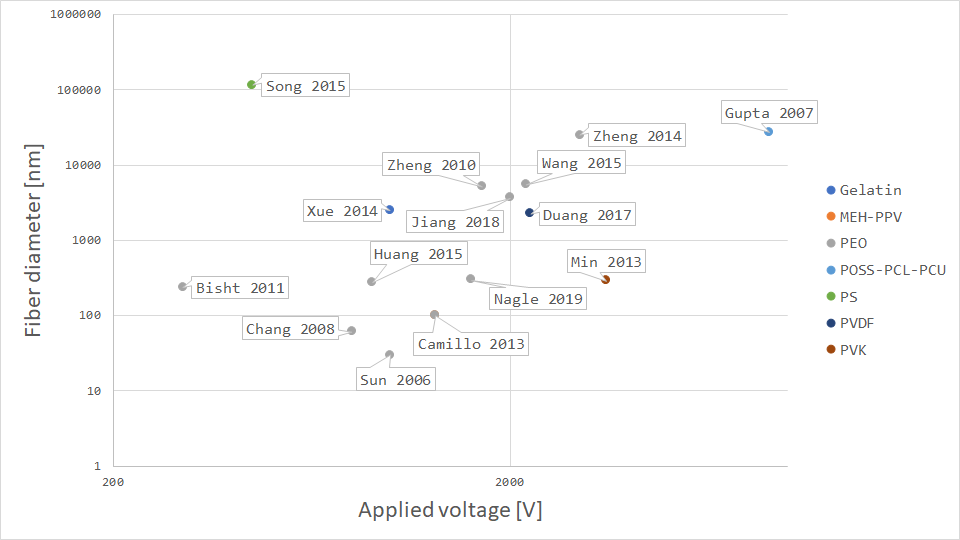
\includegraphics{images/e4441f91-c9b9-48f1-a3ed-5ec3e5033092-uplt_diametervolage.png}}{}
\makeatother 
\caption{{Applied volage vs. Fiber diameter}}
\label{f-59ed68f95344}
\end{figure*}
\egroup

\bgroup
\fixFloatSize{images/6198525c-7b44-494e-a092-206ecb3c8f9c-uweightdiameterplot.png}
\begin{figure*}[!htbp]
\centering \makeatletter\IfFileExists{images/6198525c-7b44-494e-a092-206ecb3c8f9c-uweightdiameterplot.png}{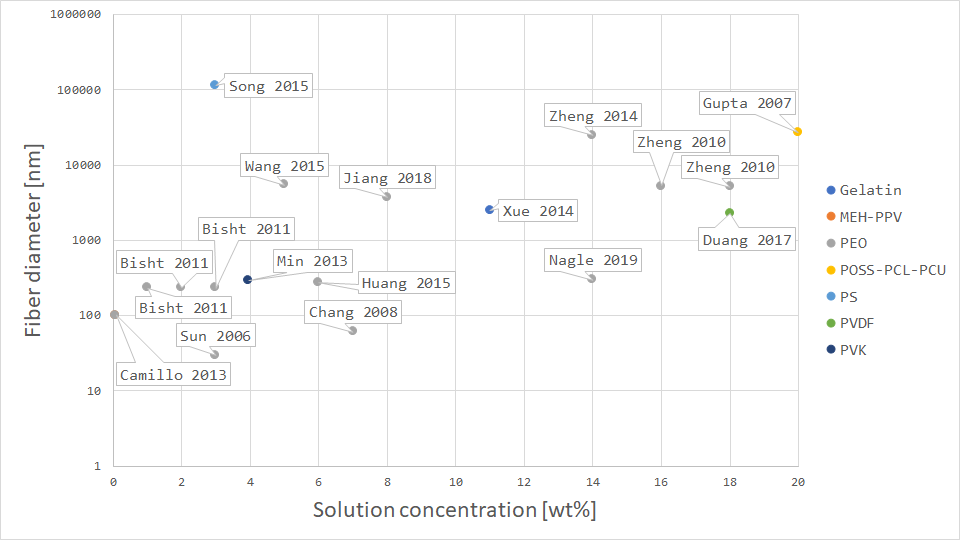
\includegraphics{images/6198525c-7b44-494e-a092-206ecb3c8f9c-uweightdiameterplot.png}}{}
\makeatother 
\caption{{Solution concentration vs. Fiber diameter}}
\label{f-0ba4df766d66}
\end{figure*}
\egroup

\bgroup
\fixFloatSize{images/fbd73f28-2c70-4a0a-be0b-f58ca8eab694-uweightconcentrationplot.png}
\begin{figure*}[!htbp]
\centering \makeatletter\IfFileExists{images/fbd73f28-2c70-4a0a-be0b-f58ca8eab694-uweightconcentrationplot.png}{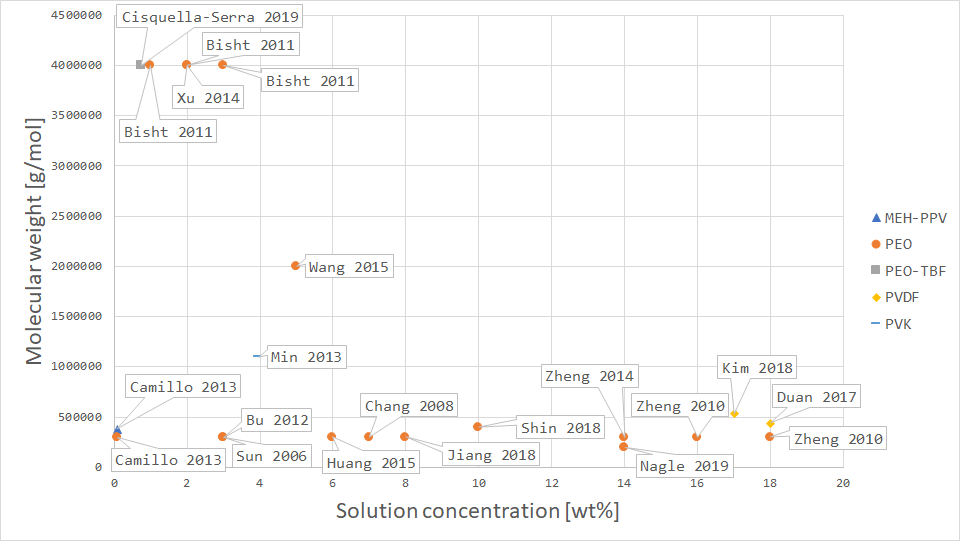
\includegraphics{images/fbd73f28-2c70-4a0a-be0b-f58ca8eab694-uweightconcentrationplot.png}}{}
\makeatother 
\caption{{Solution concentration vs. Molecular weight}}
\label{f-ab38f7e015f7}
\end{figure*}
\egroup

    
\section{NFES Achievements \& Challenges}
Lorem ipsum dolor sit amet, consectetur adipiscing elit, sed do eiusmod tempor incididunt ut labore et dolore magna aliqua. Ut enim ad minim veniam, quis nostrud exercitation ullamco laboris nisi ut aliquip ex ea commodo consequat. Duis aute irure dolor in reprehenderit in voluptate velit esse cillum dolore eu fugiat nulla pariatur. Excepteur sint occaecat cupidatat non proident, sunt in culpa qui officia deserunt mollit anim id est laborum.
\apptocmd{\thebibliography}{\csname phantomsection\endcsname\addcontentsline{toc}{section}{\numberline{}\refname}}{}{}
    



\bibliographystyle{elsarticle-num}

\bibliography{\jobname}

\end{document}
